\chapter{Сацыяльны статус}

\section{Воля да сілы}

Старажытнагрэцкі філёзаф Плятон напісаў: «Найвялікшае дабро~--- здароўе, на другім месцы~--- прыгажосьць, на трэцім~--- багацьце». З тых даўніх часоў людзі не асабліва зьмяніліся: як толькі чалавек здавальняе базавыя патрэбы ў~ежы і сьне, ён пераключаецца на здавальненьне сваіх сацыяльных запатрабаваньняў. Бо для нас, як істот сацыяльных, больш высокі статус значыць большы доступ да рэсурсаў, а~значыць і большую імавернасьць выжываньня. Думкі пра кар'еру, дастатак і зьдзяйсьненьні заўсёды прыемныя і матывуюць нас.

Калі ўзяць самага зацюканага пеўня і прыляпіць на ягоную галаву буйны яркі грэбень, то яму адразу пачынаюць саступаць першае месца ля кармушкі і аказваць знакі ўвагі. Тэма павышэньня сацыяльнага статусу для людзей таксама неймаверна важная, а~любыя пагрозы статусу, нават уяўныя, успрымаюцца вельмі гостра. Нават намёк на тое, што ``мы не крутыя, некампэтэнтныя'', моцна хвалюе, выклікаючы ``статусную трывожнасьць''.

\emph{Будучы на падпітку, навакольныя толькі й гавораць, што пра свой або чужы статус: ``Ты мяне паважаеш?'', ``Ты ведаеш, хто я?'', ``Ты ведаеш, хто мае сябры?''}

\textbf{Сацыяльны статус}~--- гэта становішча чалавека ў~грамадстве, адзін з~найважнейшых рэсурсаў здароўя. Эвалюцыйна ў~нас выпрацаваліся дастаткова дакладныя мэханізмы ацэнкі статусу як іншых людзей, так і свайго, мы аўтаматычна мяняем свае паводзіны ў~залежнасьці ад таго, як ацэньваем свой статус і як ацэньваюць наш статус іншыя людзі.

\infobox{Вылічыць нечае становішча ў~соцыуме вельмі лёгка~--- людзі заўсёды больш глядзяць на таго, хто мае вышэйшы статус.}

\textbf{Калі ў~вас высокі сацыяльны статус}, вы карыстаецеся аўтарытэтам, вашае меркаваньне мае значэньне. Калі вы гаворыце, вас уважліва слухаюць і глядзяць на вас. Вашыя прапановы падтрымліваюць і прымаюць аргумэнтацыю. Вас лічаць небясьпечным і крыху пабойваюцца, вы можаце пастаяць за сябе і, у~выпадку неабходнасьці, нанесьці страты ворагам і супернікам. Вы робіце шмат карыснага і незаменныя для каманды. З камандай вы на адной хвалі, кажаце ``мы'' і разумееце пачуцьці іншых. Вы вытрымліваеце канфліктныя сытуацыі і ня схільныя імгненна саступаць. Вы адчуваеце сваё права выказваць і мець меркаваньне, даваць свае адзнакі і абараняць свае асабістыя каштоўнасьці. У вас добрая самаацэнка, вы нават здаяцеся сабе вышэйшымі і мацнейшымі, чым ёсьць насамрэч. У стрэсавай сытуацыі вы трымаеце паставу і паднятую ўгару галаву. Вам, у~прынцыпе, здаецца, што навакольныя глядзяць на вас з~захапленьнем і ўхвалай. Пасьля стрэсу вы хутка супакойваецеся і любіце мірыцца і дамаўляцца.

\begin{figure}[htb!]
  \centering
  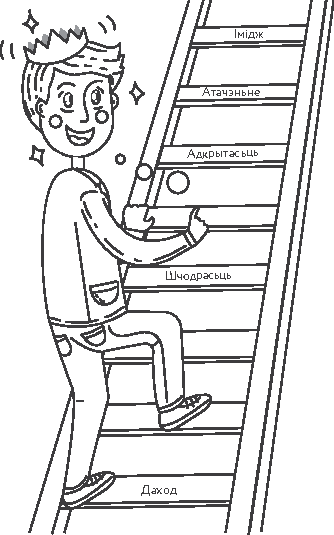
\includegraphics[scale=1.5]{willpower/ch9/1.pdf}
\end{figure}

\textbf{Калі ў~вас нізкі сацыяльны статус}, то заўважыць гэта таксама даволі проста. Калі вы гаворыце, вас ня слухаюць і на вас не глядзяць. Вашым меркаваньнем грэбуюць ці забываюць пра вас. Калі вы нешта прапануеце, гэта рэдка сустракае разуменьне і зацікаўленасьць. Іншыя ўспрымаюць вас як пухнатага і бяскрыўднага чалавека, які ня можа нашкодзіць. Вас лёгка замяніць у~калектыве, бо нічога важнага вы ня робіце. У размове вы часьцей гаворыце «я», сфакусаваныя на сваіх унутраных перажываньнях. Зь цяжкасьцю вытрымліваеце позірк, аддаеце перавагу адыходу ад канфліктных сытуацый: лягчэй падпарадкавацца, чым адстойваць свае ідэі. У канфліктнай сытуацыі вам хочацца схавацца, сьціснуцца, схіліць галаву, каб вас не заўважылі. Вы баіцеся ацэньваць, прыслухоўваецеся да думак іншых ды ідзяце ``ў іх на шворцы''. У вас нізкая самаацэнка, вы здаяцеся сабе маленькімі і слабымі, і ёсьць адчуваньне, што навакольныя глядзяць на вас з~падазрэньнем ці няўхвальна. Канфлікты надоўга выбіваюць вас з~каляіны, і вам складана аднавіцца.

\textbf{У розных культурах і розных клясах} стаўленьне да павышэньня статусу прыкметна адрозьніваецца. Але шлях героя, пераадоленьне сябе і сваіх страхаў, разьвіцьцё навыкаў, дарога да лідэрства~--- гэта важная частка дыскурсу ад антычных часоў да сучаснага заходняга сьвету. Пры гэтым пазыцыя ``не высоўвацца'' і ``быць як усе'' нам таксама добра знаёмая.

\emph{У адной антычнай гісторыі на пытаньне дыктатара, як захаваць уладу, мудрэц узяў серп і зрэзаў усе высокія каласы на полі, падраўняўшы яго. Так і таталітарныя рэжымы імкнуцца ўсярэдніваць грамадзян. Войны, рэпрэсіі, культ бедных і прыгнечаных, страх падацца заможным пад пагрозай рэпрэсій за доўгія гады глыбока ўеўся ў~сьвядомасьць людзей. Мне расказвалі, што ў~вёсках сяляне стараліся пабудаваць дом горш, чым маглі і хацелі, каб не прыцягваць да сябе ўвагу, баючыся раскулачваньня. Такая адваротная сэлекцыя пасеяла страх вылучацца, страх зарабляць, страх публічнасьці. Выраз «ты што, самы разумны?», на жаль, у~нашай культуры часьцей зьяўляецца абразай, а~не камплімэнтам.}

\infobox{Як толькі мы задавальняем базавыя патрэбы, пераключаемся на задавальненьне сваіх патрэбаў сацыяльных. Больш высокі статус значыць большы доступ да рэсурсаў, а~значыць~--- і большую імавернасьць выжываньня.}

Наша адукацыя, прафэсійная кар'ера, узровень даходу, прывабнасьць і посьпех уплываюць на ўсе сфэры жыцьця. Але проста імкненьне да ўлады разбуральнае~--- статус нараджаецца з~нашых рэальных навыкаў і дзеяў, а~спробы пераканаць іншых у~сваёй крутасьці выклікаюць адно насьмешкі. Статус~--- гэта не прыроджаная рыса, ён можа мяняцца на працягу жыцьця і вельмі хутка. Многія людзі атрымліваюць статус выпадкова, але пры гэтым яны не разумнейшыя і ня здольнейшыя, хоць і актыўна спрабуюць пераканаць у~сваёй выключнасьці астатніх.

Імкненьне да ўлады, адукацыі, прыгажосьці й багацьця~--- гэта прыродны базавы інстынкт, і ў~ім няма нічога ганебнага. Ня трэба слухаць тых, хто пераконвае нас заставацца паслухмянымі ці пакорлівымі, верыць «багатым дзядзькам», вызначае за нас наш лёс. Дзейце актыўна і верце ў~сябе. Станавіцеся мацнейшымі, разумнейшымі, багацейшымі і ўплывовейшымі, гэта палепшыць вашае здароўе і падоўжыць жыцьцё.

\textbf{Кампанэнты статусу} зьвязаныя адзін з~адным і актывуюць адзін аднаго. Так, цяпер структура стройнага і падцягнутага цела зьяўляецца адным з~ключавых паказьнікаў сацыяльнага статусу чалавека. Успрыманьне статуту адбываецца на падкорцы, літаральна ў~першыя сэкунды знаёмства, а~ад ацэнкі статуту залежыць і камунікацыя, і разьмеркаваньне рэсурсаў. Мы жывём у~час багацьця рэсурсаў і магчымасьцяў. Нам ня трэба малаціцца зь іншымі людзьмі за драбкі ежы, выракаючы іх на голад. У сьвеце ёсьць мільёны нішаў, дзе мы можам быць пасьпяховымі. Мы можам канкураваць і самі з~сабой~--- становячыся лепшымі за сябе ўчорашніх, кідаючы выклік самому часу.

\subsection*{Пытаньні і заданьні}

1. Як вы ставіцеся да публічных выступаў? Ацаніце ступень сваёй харызмы.

2. Спытайце сябе, у~чым вы можаце быць лепымі за ўсіх у~сьвеце?

3. Ці хочаце вы стаць багацейшымі, прыгажэйшымі, разумнейшымі? Што вы для гэтага зрабілі? Ці сталі вы багацейшымі, прыгажэйшымі, разумнейшымі за мінулы год?


\section{Сацыяльны статус і герархія}

Усе мы падсьвядома вельмі дакладна ўмеем вызначаць статус па вонкавым выглядзе, паставе, голасу, міміцы і да т.~п. Нават па фатаграфіі з~абліччам~--- без кантэксту адзеньня, аксэсуараў і інтэр'еру~--- мы можам ацаніць яго. З чаго ж складаецца статус? Ён уключае становішча ў~грамадстве, узровень адукацыі, улады, даходу і шэраг іншых паказьнікаў. У чалавека ёсьць як прыроджаны статус (пол, раса, нацыянальнасьць і да т.~п.), так і набыты, які дасягаецца з~дапамогай асабістых намаганьняў. Статус шчыльна зьвязаны з~выжываньнем і ўзроўнем стрэсу, а~добры прыбытак дазваляе камфортней жыць, лепей харчавацца, больш часу надаваць здароўю і выгляду, вытрачаць сродкі на даражэйшае лячэньне і т.~п.

\subsection*{Першарадны статус}

У кожнага чалавека ёсьць свой першарадны статус~--- той, які, у~асноўным, вызначае ягонае кола камунікацыі і шэраг іншых статусаў, так званы статусны набор. Першарадны статут чалавека часьцей за ўсё зьвязаны зь яго працай і складаецца зь ягонага становішча ў~працоўнай герархіі, аўтарытэт, прыбытак і прэстыж працы. Таксама вылучаюць і іншыя статусы: якое месца чалавек займае ў~сям'і, сярод сваіх сяброў, у~сваім коле па інтарэсах і да т.~п. Часам можа ўзьнікаць статусная несумеснасьць, калі ў~адной групе чалавек займае высокі ранг, а~ў іншай нізкі.

\subsection*{Адносны статус}

Для чалавека яго адносны статус у~групе нашмат важнейшы, чым абсалютны. У дасьледаваньнях людзі згаджаліся мець меншы ўзровень даходу ці менш прывабны выгляд, калі пры гэтым у~навакольных будзе яшчэ менш грошай. І не згаджаліся на сытуацыі, дзе яны станавіліся б багацейшымі ці прыгажэйшымі, але ў~асяродзьдзі яшчэ багацейшых і прыгажэйшых.

\emph{Калі Юлій Цэзар праяжджаў празь невялікі горад, то заўважыў, што ``лепей быць першым тут, чым другім у~Рыме''.}

\infobox{Для многіх людзей спробы павысіць свой статус там, дзе большасьць атачэньня мае вышэйшы статус, ды да таго ж і прыроджаны, могуць быць шкодныя для здароўя.} 

Калі б вы нічога не мянялі ў~сваім жыцьці, але былі акружаны людзьмі з~ніжэйшым статусам, то ваш узровень стрэсу зьнізіўся б, а~працягласьць жыцьця~--- павялічылася. Такім чынам, нашмат важней, як ацэньваеце сябе вы і навакольныя~--- вас. Калі вы лічыце сябе багатым~--- усё выдатна. Калі вы багатыр, але баіцеся ўсё страціць, ці вашыя сябры зарабляюць на парадак вышэй, то тады гэтыя грошы наўрад ці пойдуць вам на карысьць.

\textbf{Суб'ектыўны статус}~--- гэта ўнутранае адчуваньне сваёй значнасьці і ўлады. Уплыў суб'ектыўнай ацэнкі сацыяльнага статусу на здароўе і працягласьць жыцьця большы, чым у~аб'ектыўнай. Чалавек з~высокім становішчам, але пакутамі ад адчуваньня сваёй нікчэмнасьці, магчыма, будзе мець больш рызыкаў для здароўя, чым бяздомны ў~начлежцы, які карыстаецца аўтарытэтам і ўладай. 

\textbf{Невыпадкова такая, здавалася б, неадаптыўная копінг-стратэгія, як самаўзвышэньне, валодае карысным узьдзеяньнем на здароўе. Але стварэньне ілюзій~--- гэта як абязбольваньне, якое ня лечыць, а~толькі маскіруе сымптомы і пасуе адно для часовых мер.}

\subsection*{Першабытная роўнасьць}

Людзі маюць некалькі стратэгіяў арганізацыі ўзаемадзеяньня ў~групах. Найстаражытнейшая праграма~--- гэта герархія, сацыяльная лесьвіца з~вызначэньнем выразнага становішча кожнага чальца. Пры гэтым прасоўваньне магчымае толькі з~дапамогай барацьбы. Але з~пункту гледжаньня эфэктыўнасьці такія праграмы ня надта адаптыўныя і захаваліся ў~сучасным сьвеце адно ў~сілавых ведамствах.

\emph{Калі ў~старажытных зьявіліся віды зброі, здольныя забіць на адлегласьці,~--- такія як дзіда і лук,~--- то грубая фізычная сіла стала мець меншае значэньне, і людзі пачалі дамаўляцца. Нашыя продкі, у~адрозьненьне ад іншых прыматаў, навучыліся дзеяць кааліцыямі, выпрацоўваць агульныя пляны дзеяў. Аўтарытэт у~плямёнах грунтаваўся на прынцыпе роўнасьці без падпарадкаваньня аўтарытарнаму лідэру. Такая салідарнасьць племя была важная, бо індывідуальнае супрацьстаяньне важаку, вядома, небясьпечнае.}

Эгалітарызм, або роўнасьць, узьнікшы ў~паляўнічых-зьбіральнікаў, стаў часткай чалавечай культуры. Сфармаваліся плюралістычныя мадэлі, пры якіх людзі дамаўляюцца дзеяць, датрымліваючыся правілаў і захоўваючы павагу адно да аднаго.

\subsection*{Герархія}

Тым ня менш старажытныя інстынкты працягваюць моцна на нас уплываць. У сучасным грамадстве людзі, трапляючы ў~групы, аўтаматычна арганізуюцца ў~сацыяльныя структуры. Умоўна можна вылучыць альфа-паводзіны, бэта і амега. Становішча чалавека ў~герархіі залежыць ад прыроджаных якасьцяў (напрыклад, генэтыка і ўзровень унутрычэраўнага тэстастэрону) і яго навыкаў (стрэсаўстойлівасьць, сацыяльныя навыкі і інш.). Некаторыя людзі марнуюць усе сілы на прасоўваньне уверх па сацыяльнай лесьвіцы, іншым гэта менш цікава. Найважнейшым крытэрам посьпеху зьяўляецца сіла перакананасьці ў~сваёй перавазе і праве на ранг, а~таксама зацятасьць і настойлівасьць. Чым мацнейшая гэтая перакананасьць, тым лягчэй чалавек трывае канфлікты. А вось калі ў~чалавека такой упартасьці або ўпэўненасьці няма, то ён адчувае моцны дыскамфорт ад канфлікту, і яму прасьцей здацца ці адмовіцца ад канкурэнцыі.

\emph{У кожным з~нас закладзены страх высоўвацца, і гэта не выпадкова. Бо ва ўмовах герархіі, калі ідзе жорсткая канкурэнцыя, адрозьнівацца~--- гэта значыць кінуць выклік важаку. Выклік мае на ўвазе бітву да сьмерці або выгнаньне таго, хто прайграў, са зграі, як гэта бывае ў~малпаў. У такім разе быць амэгай выгадна, бо гэта дапамагае выжыць.}

\begin{figure*}[htb!]
  \centering
  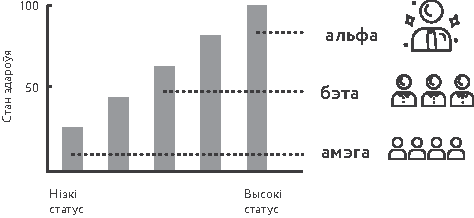
\includegraphics[scale=1.5]{willpower/ch9/2.pdf}
\end{figure*}

\textbf{Альфы} імкнуцца актыўна ўплываць на навакольны сьвет, правакуюць канкурэнцыю ды імкнуцца да перамогі, праяўляюць актыўную агрэсіўнасьць. Для альфы характэрны прыўзьняты настрой, харызматычнасьць, паблажлівасьць, просталінейнасьць, выклік, паядынак па ясных правілах і сумленнасьць. Альфы намагаюцца максімальна пашырыць свой уплыў і нарасьціць сваю сілу. Пры гэтым альфы эгаістычныя, могуць быць асацыяльнымі і дэструктыўнымі, адмаўляюцца падпарадкоўвацца правілам, калі самі не зацікаўленыя ў~іх выкананьні. Бяруць на сябе адказнасьць, ствараюць нешта арыгінальнае і ўнікальнае, імкнуцца стаць незалежнымі ад свайго асяродзьдзя і яго ацэнак.

\textbf{Амэгі} больш заклапочаныя тым, каб лепей пачувацца і рабіць уражаньне на навакольных, ім вельмі важна тое, як яны выглядаюць збоку. Пазьбягаюць канкурэнцыі і дазваляюць іншым быць актыўнымі, адмаўляюцца мяняць нешта ў~навакольным сьвеце і складзенай сыстэме правілаў. Амэгі маюць дрэнную сацыяльную інтуіцыю. Для іх характэрныя эмацыйная нестабільнасьць, трывожнасьць, нежаданьне даваць свае асабістыя ацэнакі ці прытрымлівацца вызначаных прынцыпаў. Больш схільныя да пасіўнай агрэсіі, ныцьця ці абурэньня, лічаць сябе ахвярай. Да станоўчых бакоў амэгаў можна аднесьці дысцыплінаванасьць, неканфліктнасьць, сьціпласьць і падпарадкаваньне правілам. Яны імкнуцца быць як усе, залежаць ад калектыву і прытрымліваюцца чужых правілаў. Пры гэтым пастаянна абсякаюць тых, хто спрабуе вылучыцца ці мае меркаваньне, адрознае ад меркаваньня большасьці.

\textbf{Бэты} займаюць прамежкавае становішча. У іх адсутнічаюць дакладныя правілы і мэты, як у~альфаў, але яны імітуюць іх, спрабуючы прэтэндаваць на ролю лідэраў. Бэты імкнуцца забясьпечыць сабе камфорт праз пазітыўнае асяродзьдзе, стварэньне ілюзіі лідэра празь сьвіту, адзеньне і да т.~п. Яны пазьбягаюць адказнасьці і перакладаюць працу на іншых людзей, пры гэтым забіраючы рэсурсы групы. Як і амэгі, бэты ў~першую чаргу думаюць аб тым, як спадабацца іншым і ўразіць іх.

\subsection*{Пытаньні і заданьні}

1. Ці ацэньваеце вы самі розныя ідэі, рэчы і людзей ці імкняцеся спачатку даведацца чужое меркаваньне?

2. Які ваш першарадны статус? Якія яшчэ статусы ў~вас ёсьць? Як вы сябе ацэньваеце суб'ектыўна і ці адрозьніваецца гэтая ацэнка ад меркаваньня навакольных?

3. Ці лёгка вам вытрымліваць сутыкненьні і канфлікты?


\section{Уплыў на здароўе. Чаму ў~пераможцаў хутчэй гояцца раны?}

Высакастатусныя жывёлы адрозьніваюцца дагледжанасьцю, ярчэйшай афарбоўкай, буйнейшымі грабянямі, ікламі, плаўнікамі і да т.~п. Гэтак жа і ў~людзей~--- чым вышэйшы статус, тым менш у~яго праблемаў са здароўем, лепшы выгляд і вышэйшая працягласьць жыцьця. Сацыяльны статус~--- гэта незалежны рэсурс здароўя чалавека, і яго ўплыў мы часта недаацэньваем. 

Сацыяльны статус уплывае на стан здароўя мноствам спосабаў. З аднаго боку, гэта доступ да лепшай мэдыцыны, умоваў жыцьця (паветра, дом, шум), меншы ўзровень стрэсу, больш здаровы лад жыцьця і сацыяльнага асяродзьдзя і т.~п. У дасьледаваньнях вывучаюцца канкрэтныя мэханізмы ўплыву сацыяльнага статусу на актыўнасьць сымпатаадрэналавай сыстэмы, імуннай сыстэмы і нават актыўнасьць генаў.

\subsection*{Мозг і статус}

Сацыяльны статус пачынае ўплываць на нас з~самага дзяцінства, нават нараджэньне ў~беднай сям'і аўтаматычна павялічвае рызыку для здароўя. Дзеці зь бяднейшых сем'яў горш вучацца, іх маўленьне разьвіваецца павольней. Нізкі сацыяльны статус бацькоў уплывае на мозг: вядзе да зьмены абмену сэратаніну, што павялічвае рызыку дэпрэсіі, павялічвае актыўнасьць мігдалападобнага цела, а~гэта, у~сваю чаргу, павялічвае трывожнасьць і зьмяншае стрэсаўстойлівасьць. У дзяцей, бацькі якіх атрымалі вышэйшую адукацыю, плошча кары галаўнога мозга на 3\,\% большая ў~параўнаньні зь дзецьмі, бацькі якіх вышэйшай адукацыі не атрымалі.

\textbf{Павышэньне статусу, атрыманьне славы і прызнаньня~--- гэтае пачуцьцё любяць усе людзі ва ўсім сьвеце. Рост статусу павышае ўзровень дафаміну, сэратаніну і тэстастэрону, а~картызол пры гэтым зьніжаецца.}

Калі ўзровень дафаміну ў~галаўным мозгу павялічваецца, чалавек ясьней думае, у~яго вышэйшыя актыўнасьць прэфрантальнай кары, нэўраплястычнасьць і кантроль эмоцыяў, канцэнтрацыя. Гэта робіць яго яшчэ больш актыўным, фармуючы станоўчую зваротную сувязь, як у~прымаўцы: ``Бедныя бяднеюць, а~багатыя багацеюць''.

\subsection*{Стрэс}

Чым ніжэй статус, тым вышэй узровень АКТГ і картызолу. Людзі зь нізкім статусам больш нэрвовыя, горш спраўляюцца са стрэсам і мацней на яго рэагуюць. Людзі з~больш высокім статусам адчуваюць большы ўзровень кантролю і ўлады, а~значыць лягчэй даюць рады стрэсу і лепш вядуць справы. Стрэсаўстойлівасьць дазваляе рабіць тое, чаго баісься, выходзіць з~зоны камфорту.

\textbf{Пры ўзьдзеяньні аднолькавага стрэсара пульс пачашчаецца мацней у~тых, у~каго ніжэйшы статус.} Нізкі статус зьвязаны зь вялікай колькасьцю адмоўных эмоцыяў, бо наймацнейшым нэгатыўным мэханізмам дзеяньня беднасьці зьяўляецца пастаянны стрэс, часта некантраляваны. Больш высокі сацыяльны статус зьвязаны як зь меншым узроўнем трывожнасьці, так і зь ніжэйшым узроўнем запаленьня ў~арганізьме.

\subsection*{Перамога}

Перамога ня толькі павышае ўзровень тэстастэрону, але й павышае адчувальнасьць розных аддзелаў мозгу да ўзьдзеяньня тэстастэрону. Любая перамога~--- у~шахматах, у~відэагульні або ў~бізнэсе~--- павышае ўзровень тэстастэрону. 

\emph{Перамога павялічвае шчыльнасьць рэцэптараў тэстастэрону ў~ядры ложа канчатковай палоскі, што ўплывае на сувязь прэфранталка-мігдаліна, і ў~дафамінавых структурах (прылеглае ядро і вэнтральная покрыўка), што павялічвае выдзяленьне дафаміну ў~адказ на павышэньне тэстастэрону.}

\textbf{Сацыяльны градыент}~--- гэта адрозьненьні ў~стане здароўя, зьвязаныя са зьменай становішча на герархічнай лесьвіцы. Даведзена, што статус~--- гэта незалежны чыньнік рызыкі хваробы. Чым ваш статус вышэйшы, тым меншая рызыка дэпрэсіі і сардэчна-сасудзістых захворваньняў. Пры нізкім статусе сардэчна-сасудзістыя хваробы пачынаюцца раней і працякаюць больш агрэсіўна~--- такім людзям патрабуецца і больш стараннае лячэньне.

\emph{У пераможцаў раны гояцца хутчэй~--- гэта было вядома яшчэ ў~антычныя часы. Дасьледаваньні на малпах пацьвердзілі, што гэта сапраўды так.}

\begin{figure}[htb!]
  \centering
  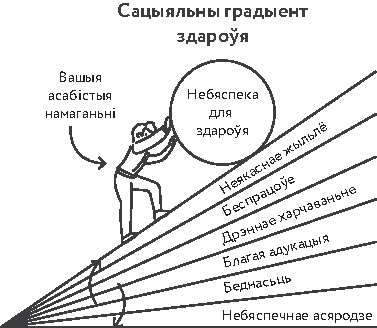
\includegraphics[scale=1.2]{willpower/ch9/3.pdf}
\end{figure}

\subsection*{Парадокс шкоды алькаголю}

Бядняк~--- адэпт здаровага ладу жыцьця хварэе часьцей за пітушчага багацея-курца. Вядома, што людзі з~высокім і нізкім сацыяльна-эканамічным статусам п'юць аднолькава, але рызыка сьмерці, зьвязаная з~ужываньнем алькаголю, вышэйшая ў~нізкастатусных.

\emph{Пры вывучэньні сардэчна-сасудзістых хваробаў высьветлілася, што багатыя высокаадукаваныя амэрыканцы, якія п'юць, кураць і не займаюцца спортам, радзей пакутуюць на сардэчна-сасудзістыя захворваньні, чым бедныя неадукаваныя амэрыканцы, якія робяць тое ж самае. Колькасьць інфарктаў і інсультаў у~беднякоў, якія займаліся спортам, не курылі і не пілі, аказалася нават вышэйшай, чым у~багацеяў з~усімі чыньнікамі рызыкі.}

\textbf{Імунітэт.} Нізкі статус сёньня~--- гэта не прысуд. Статус мяняецца хутка, разам зь ім мяняецца і яго ўплыў на здароўе. Змяненьне статусу ўплывае на актыўнасьць каля тысячы генаў. Даведзена, што павышэньне сацыяльнага статусу можа зьмяніць нашу імунную сыстэму, зьнізіць канцэнтрацыю гармонаў стрэсу і паменшыць запаленьне.

\infobox{Навукоўцы могуць вызначыць месца макакі ў~герархіі нават па аналізе яе крыві.}

У дасьледаваньні навукоўцы крапалі добраахвотнікам у~нос вірус грыпу або рынавірус і адпраўлялі іх на карантын. Аказалася, што чым вышэй чалавек ацэньваў (суб'ектыўна) сваё сацыяльна-эканамічнае становішча, тым менш у~яго была рызыка заражэньня. Магчыма, гэта зьвязана з~тым, што больш высокі статут спалучаны зь лепшым сном, меншым стрэсам і лепшым станам імунітэту.

\subsection*{Працягласьць жыцьця}

Невыпадкова кажуць, што найлепшы герапратэктар~--- гэта багацьце. Самыя вялікія і дарагія помнікі стаяць на магілах доўгажыхароў.

\emph{У ЗША розьніца ў~працягласьці жыцьця паміж багатымі і беднымі перавышае 15 гадоў для мужчынаў і 10 гадоў для жанчынаў. Цікава, што ў~бяднейшых краінах зь меншым узроўнем няроўнасьці такой моцнай розьніцы няма.}

Ацэнка біялягічнага ўзросту ў~блізьнятаў паказала, што няўдалая ў~жыцьці сястра-блізьня на 7 і больш гадоў была біялягічна старэйшая за сваю пасьпяховую сястру. Сярод актораў Галівуду даўжэй жывуць уладальнікі Оскара~--- у~сярэднім на 3 гады. Усяго толькі 4 гады беднасьці на працягу жыцьця ўжо прыводзяць да заўчаснага старэньня, што праяўляецца ў~горшых паказьніках тэстаў на трывушчасьць.

\subsection*{Пытаньні і заданьні}

1. Ня зайздрасьць, а~натхненьне. Хто зь людзей з~высокім статутам вас натхняе? Як яны яго дамагліся?

2. Пачніце весьці дзёньнік перамог. Запішыце і перажывіце зноў усе вашыя дасягненьні.

3. Зрабіце сабе куток пераможцы. Зьбярыце ўсе граматы, дыплёмы, фота, усе доказы пасьпяховасьці з~самых раньніх гадоў.


\section{Псыхалёгія сацыяльнага статусу}

Нізкі статус выракае нас на нізкія даходы, адсутнасьць магчымасьці выбіраць працу, асяродзьдзе, спосаб баўленьня часу. Адчуваньне безвыходнасьці, якое ўзьнікае пры немагчымасьці зьмяніць свой статус, штурхае на пошукі дафамінавай «халявы»: людзі больш кураць, п'юць і ў~цэлым менш клапоцяцца пра здароўе, іх гарызонт плянаваньня звужаецца. Навошта ж жыць, калі надзеі няма? Нізкастатусныя людзі часьцей сутыкаюцца з~прыніжэньнем і цкаваньнем, у~іх часьцей узьнікаюць кагнітыўныя парушэньні, сардэчна-сасудзістыя захворваньні, зьніжэньне фэртыльнасьці.

\infobox{Высокі сацыяльны статус~--- гэта ня проста карысна, але яшчэ й вельмі прыемна.}

Цешыць нават надзея на павышэньне статусу. Невыпадкова людзі так любяць гісторыі пра папялушак і супергерояў, гэтая тэма ёсьць у~мностве літаратурных твораў. Зрэшты, ня трэба занадта імкнуцца. Існуе эфэкт ``поўнага правалу'', сутнасьць якога ў~тым, што той, хто памыляецца й часам робіць глупствы, больш падабаецца людзям, чым той, хто не памыляецца ніколі.

\emph{Яшчэ з~антычных часоў слава~--- гэта рухальная матывацыя герояў.}

З даўніх часоў людзі любяць расказваць гісторыі, у~якіх звычайны чалавек становіцца героем. Як правіла, гэта чалавек зь нізкім статусам, які атрымлівае заданьне і залучаецца ў~ланцужок падзей. У працэсе ён атрымлівае дапамогу, праходзіць навучаньне ў~мудраца ці багіні, пераадольвае чараду спакусаў і выпрабаваньняў, у~працэсе чаго атрымлівае досьвед. Затым адбываецца фінальная бітва са злом, сьмерць і ўваскрашэньне героя ў~іншасьвеце. Пасьля гэтага ён атрымлівае ўзнагароду і жонку, ягоны статус падвышаецца, і ён вяртаецца дамоў, каб дапамагчы іншым людзям і жыць доўга і шчасьліва. \textbf{Што ж, гэтыя гісторыі прынамсі вучаць нас, што для падвышэньня статуту трэба пастарацца!}

\subsection*{«Візуальны статус»}

У шматлікіх плямёнах паляўнічых-зьбі\-раль\-ні\-каў правадыру важней раздаваць падарункі і ежу, каб здабыць павагу супляменьнікаў, а~не назапашваць іх для абмену ці продажу. Пошук павагі і прызнаньня~--- гэта частая рухальная сіла нашых учынкаў. Чым ніжэйшы статус, тым мацней хочацца яго ўзьняць. А вось людзі з~больш высокім статусам адчуваюць меншую неабходнасьць яго даводзіць. Так, чым ніжэйшы статус, тым мацней мужчына заклапочаны давядзеньнем мужнасьці і нават часьцей ходзіць у~спартовую залю.

Нізкі статус суправаджаецца адчуваньнем безвыходнасьці і штурхае нас на пошукі лёгкіх спосабаў атрыманьня задавальненьня~--- алькаголь, наркотыкі і інш. Мы менш клапоцімся пра сябе і сваё здароўе, бо навошта жыць, калі надзеі няма?

Паняцьці ``сіла'' і ``статус'' не заўсёды ідэнтычныя. У ідэальным сьвеце ўнутраная сіла чалавека (рэальны кантроль каштоўных рэсурсаў і ўменьняў) зьвязаная зь ягоным статусам (павага, якую чалавек атрымлівае ад іншых пры дэманстрацыі сваіх навыкаў). Але статус можна хутка падняць з~дапамогай адмысловых дэманстратыўных сыгналаў, як біялягічных, так і сацыяльных (``крутое аўто'', ``уплывовыя сябры'' і інш.). Калі чалавек пачуваецца бясьсілым, то ён спрабуе гэта кампэнсаваць, зьвяртаючыся дзеля павышэньня сацыяльнага статуту да мноства пацешных рэчаў. Напрыклад~--- купля рэчаў большага памеру для візуальнага павелічэньня цела.

\textbf{Велізарная хата, велізарны тэлевізар, велізарная машына}~--- усё гэта спробы дэманстрацыі статуту. Вельмі часта людзі зь нізкім статусам яшчэ больш пагаршаюць свой фінансавы стан, спрабуючы зрабіць уражаньне на навакольных, павялічваючы свой ``візуальны статус''~--- максімум дарагіх упрыгожаньняў і адзеньня, нават калі гэта недарэчна і выглядае вульгарна. Людзі кампэнсуюць нізкі статус шопінгам, пераяданьнем і гатовыя дзеля гэтага браць крэдыты.

\emph{Дасьледаваньні паказваюць, што калі штучна прынізіць статус чалавека, то ён гатовы заплаціць вялікую суму за ``прэстыжныя'' тавары. Чым вышэйшы ў~пакупніцы даход, тым зь меншым памерам лягатыпу яна выбірае торбу.}

Экспэрымэнтальнае зьніжэньне статусу і выкліканьне бясьсільля ў~чалавеку прыводзіла да таго, што ён выбіраў вялікія порцыі ежы, асабліва ў~прысутнасьці іншых. Людзі з~высокім статусам выбіралі меншыя порцыі пры любых абставінах, бо няма патрэбы дэманстраваць тое, у~чым яны і так упэўненыя. Чаму? У старажытнасьці той, каму даставаўся большы кавалак і ў~каго было больш тлушчу, лічыўся лепшым паляўнічым. Зь іншага боку, гэта форма дэманстратыўнага спажываньня. Людзі~--- істоты глыбока сацыяльныя, і часта нашыя дзеі можна зразумець адно праз прызму міжасобасных камунікацыяў і герархічных пасылаў.

\subsection*{Ня верце}

Цікава, што дамінаваньне ў~групе і кампэтэнтнасьць могуць быць зусім не зьвязаныя. Але нашыя кагнітыўныя скажэньні працуюць так, што словы любога чалавека з~больш высокім статутам здаюцца нам праўдзівымі, і мы схільныя яму давяраць. Мы нават лепш распазнаём эмоцыі на тварах высакастатусных людзей, чым нізкастатусных. Статус іншых уплывае на тое, будзем мы рызыкаваць ці не. Вельмі часта аўтарытэты прыгнятаюць нас: сустракаючы старэйшых па статусе, мы неўсьвядомлена ім падпарадкоўваемся, аўтаматычна лічачы іх разумнейшымі. Крытычна адсочвайце сваё жаданьне падпарадкавацца чужому статусу, пераадольвайце яго.

\emph{Паказальны экспэрымэнт зь дзьвюма клеткамі з~малпамі, у~адной зь іх~--- альфа-самец, у~іншай~--- амэга. Калі амэгу пакласьці банан у~клетку, то ён будзе баяцца ўзяць яго, асьцерагаючыся адплаты. Але калі завесіць клетку з~альфай тканінай, то амэга спакойна есьць банан.}

\subsection*{«Стварэньне я дрыготкае або права маю?»}

Калі мы расьцём у~спрыяльным сацыяльным асяродзьдзі, то літаральна ўбіраем яго і, у~залежнасьці ад набытага статуту, па-рознаму рэагуем на сытуацыі. Людзі з~высокім статутам у~глыбіні душы ўпэўненыя, што могуць прэтэндаваць на тое, што належыць ім па праве. Пры нізкім статусе ў~чалавека няма ўпэўненасьці, што ён наогул можа прэтэндаваць на больш высокі заробак або пасаду, ён як бы падзяляе ўсе магчымасьці на ``гэта дазволена мне'' і ``гэта недапушчальна для мяне''.

\emph{Для многіх людзей статуснай праблемай зьяўляецца іх заніжаная самаацэнка. Калі ў~вас таксічнае асяродзьдзе, якое падрывае ўпэўненасьць у~сабе, то важна зьмяніць яго на спрыяльнае. Важна перастаць выкарыстоўваць у~свой бок нэгатыўны стыль звароту (лаяць, ненавідзець сябе, абзываць ці мець нэгатыўныя ўсталёўкі), а~акрамя гэтага~--- сабраць набор пазітыўных уяўленьняў пра сябе (у чым вы добрыя, якія ў~вас ёсьць разыначкі, дасягненьні, хто і калі вас хваліў і да т.~п.). Адзначайце і запамінайце ўсё добрае, што пра вас гавораць, а~дрэннае не прымайце блізка да сэрца.}

Высакастатусныя людзі вераць: усё, што ёсьць у~сьвеце, прызначана для іх, і яны могуць гэтым карыстацца і могуць вырашыць любую задачу. Нізкастатусныя людзі лічаць, што магчымасьці~--- гэта для іншых людзей, а~яны гэтага нявартыя, і гэтыя задачы~--- невырашальныя ў~прынцыпе.

У музеі, напрыклад, высокастатусныя людзі самі даюць ацэнкі карцінам і прадметам мастацтва; калі ім нешта не падабаецца, яны могуць сказаць, што гэта ``дрэнная'' статуя або карціна. Людзі зь сярэднім статутам чытаюць даведнік і спрабуюць зразумець, якую карціну лічыць добрай, а~нізкастатусныя людзі наогул ня могуць ацаніць і выказаць сваё меркаваньне. Нашыя кагнітыўныя скажэньні працуюць так, што словы любога чалавека з~больш высокім статусам здаюцца нам праўдзівымі. Вельмі часта аўтарытэты душаць нас: мы неўсьвядомлена ім падпарадкоўваемся, аўтаматычна лічачы іх разумнейшымі.

Такая ўпэўненасьць праяўляецца ня толькі на ўзроўні думак, але й на ўзроўні цела. Больш высокі статус і ўзровень дафаміну робяць чалавека расслабленым, забясьпечваюць добры цяглічны тонус, што вядзе да лепшага валоданьня целам, прыгожай паставы, плястычнасьці рухаў. Іх дэманструюць свабодныя позы, упэўненасьць у~сабе. У сваю чаргу нізкі статус~--- гэта нязграбнасьць і заціснутасьць.

\textbf{Манэра трымацца~--- гэта агульнае ўражаньне ад становішча галавы, позірку, паставы і хады.} Уладная манэра паводзіцца, узнаўленьне моцных позаў вядзе да таго, што чалавек аўтаматычна прымярае на сябе пазыцыю лідэра. Моцныя позы зьвязаныя з~большай стрэсаўстойлівасьцю, меншым узроўнем картызолу і вялікім~--- тэстастэрону.

Вышэйшы статус дазваляе лягчэй рызыкаваць: у~выпадку посьпеху дасягаецца яшчэ больш высокі статус, а~калі здараецца няўдача, дык усё адно застаецца запас магчымасьцяў. Калі ў~чалавека ёсьць першапачатковы запас, то можна доўга шукаць і экспэрымэнтаваць, таму высокастатусныя людзі не баяцца прайграць. А калі чалавек адчувае, што ў~яго мала сілаў і магчымасьцяў, то ён не рызыкуе і выбірае больш сьціплы, але надзейны варыянт. 

\emph{Праўда, чым надзейнейшы варыянт, тым меншая магчымасьць вялікага выйгрышу.}

Чым менш рэсурсы, тым часьцей чалавек жыве адным днём, бо пры стрэсе галоўнае~--- выжыць! Нізкастатусныя людзі часта бестурботныя, бо ў~іх нізкі гарызонт плянаваньня: заробленыя грошы марнуюць на забаўкі, а~не інвэстуюць у~будучыню. Людзі, якія вырасьлі ў~такім асяродзьдзі, маюць мала шанцаў падняцца вышэй, і нават калі ў~іх зьяўляецца больш грошай, то яны працягваюць распараджацца імі як бедныя. Прыклады лятарэяў паказальныя~--- практычна ўсе лёсікі спусьцілі свае мільёны і аказаліся больш няшчаснымі, чым да выйгрышу.

\subsection*{Выпрабаваньне мядзянымі трубамі}

Выпрабаваньне ўладай~--- самае цяжкае. Калі непадрыхтаваныя людзі выпадкова прыходзяць да ўлады~--- без паступовага ўзыходжаньня, а~ў выніку прызначэньняў або крызісу,~--- улада можа сказіць іх карціну сьвету і прымусіць пакутаваць тых, хто апынуўся ніжэй у~герархіі. Павышэньне статусу павышае веру ў~сваю асаблівасьць, абранасьць і свае рашэньні, якія здаюцца адзіна слушнымі. Кіраўнікі лепш разумеюць эмоцыі іншых людзей, але яны ж адчуваюць менш эмпатыі да іх.

Нэўрабіёлягі нават кажуць пра «сындром ганарыстасьці» ці гібрыс-сындром. Тыя, хто знаходзіўся доўга ва ўладзе, часта паступалі так, як людзі з~чэрапна-мазгавой траўмай: яны былі імпульсіўныя, схільныя рызыкаваць, страчвалі эмпатыю, выяўлялі самадзейнасьць, ігнаравалі здаровы глузд. Чым даўжэй знаходзіцца чалавек ва ўладзе, тым ён мацней страчвае кантакт з~рэальнасьцю, адчувае больш пагарды да астатніх людзей, праяўляе больш некампэтэнтнасьці і паступова страчвае кантакт з~рэальнасьцю.

Як слушна кажуць, «улада разбэшчвае, а~абсалютная ўлада разбэшчвае абсалютна». У багатых людзей зь цягам часу таксама выяўляецца дэфармацыя асобы: чым багацейшы чалавек, тым больш ён схільны хлусіць і парушаць закон, браць і даваць хабары і ўхваляць неэтычныя паводзіны. 

\emph{Больш высокі статус павялічвае схільнасьць да рызыкі, у~тым ліку ня толькі ў~новых праектах, але й у~агрэсіі да навакольных, і нават рызыкі неабароненага сэксу.}

\subsection*{Пытаньні і заданьні}

1. Зь якім гераічным пэрсанажам вы сябе асацыюеце? Чаму?

2. Ці часта вы завышаеце свае здольнасьці і спрабуеце пусьціць пыл у~вочы? Памятайце, што гэта можа выклікаць нэгатыўную рэакцыю навакольных.

3. Ці падабаецца вам камандаваць? Якія эмоцыі вы пры гэтым адчуваеце?


\section{Праца і даход}

Ваша праца і ўзровень даходу~--- важная частка статусу. Першачарговы статус для большасьці людзей~--- прафэсійны. Таму нізкая пасада, непрэстыжная малааплатная пазыцыя, страта працы, выхад на пэнсію зьніжаюць сацыяльны статус. А вось прэстыжная праца, павышэньне на пасадзе, прафэсійная кампэтэнтнасьць павышаюць ня толькі статус, але й самаацэнку.

\emph{Праца~--- гэта ня проста даход, але й статус, структураваньне часу, калектыў, самаідэнтыфікацыя. Таму яе страта зьмяншае і задаволенасьць жыцьцём. Беспрацоўе павышае рызыку заўчаснае сьмерці на 63\,\%, прычым эфэкт мацнейшы для мужчынаў маладзейшых за 50 гадоў. На 60\,\% павялічваецца рызыка інсульту, у~два разы часьцей здараюцца праблемы са здароўем, у~тым ліку анкалёгія і псыхічныя захворваньні.}

Статус, прама ці ўскосна, зьвязаны з~вашымі рэсурсамі. Чым большымі рэсурсамі вы валодаеце, незалежна ад іх разнавіднасьці~--- абаяньне, харызма, уплыў, улада, грошы, сіла, рэдкія навыкі або здольнасьці, то бок усё тое, што адрозьнівае вас ад навакольных,~--- тым вышэйшы будзе ваш статус. Любыя дзеяньні, якія вядуць да росту вашае сілы й рэсурсаў, добрыя і карысныя.

\emph{Ніцшэ пісаў, што «каштоўнасьць~--- гэта найвялікшая колькасьць улады (перадусім над сабой), якую чалавек можа засвоіць».}

\subsection*{Узровень даходу}

Фінансавы стан моцна ўплывае на статус чалавека і ягонае здароўе. Гэта вельмі заўважна ў~краінах з~платнай мэдыцынскай дапамогай і меншы ўплыў мае ў~дзяржавах з~роўным доступам да мэдыцынскіх паслуг. Дастатковы ўзровень капіталу, яго правільнае ўкладаньне гарантуе вам абарону, догляд, здаровае харчаваньне і лячэньне на працягу ўсяго жыцьця.

\infobox{Падушка бясьпекі, нават пры адсутнасьці вялікіх вытратаў, дзейнічае заспакаяльна і дазваляе аптымістычна глядзець наперад. У іншай сытуацыі~--- зьмірыцеся зь няпэўнасьцю, бо лепшае, што можна зрабіць для будучыні,~--- трэніраваць сваю адаптыўнасьць.}

Што сказаць, калі нават просты мэханічны пералік грошай можа зьняць болевыя адчуваньні, спрыяючы выдзяленьню эндарфінаў. Нездарма Скрудж Макдак (герой «Качыных гісторый», качар-мільярдэр) купаўся ў~золаце! Павышайце свой узровень фінансавай пісьменнасьці, заўсёды адкладайце частку прыбытку, пазьбягайце крэдытаў і даўгоў. Фінансавыя крызісы цяжэй за ўсё ўплываюць менавіта на бедных, павялічваючы рызыкі сардэчна-сасудзістых захворваньняў, самагубстваў і да т.~п.

У наш час звыклыя працы і тыпы занятасьці перажываюць сур'ёзныя зьмены. Расьце доля анляйн-работы. Узмацняецца расслаеньне ў~даходах, зьнікае сярэдні клас. Рынак працы становіцца глябальным. Аўтаматызацыя скарачае колькасьць працоўных месцаў, а~за наяўныя ўзрастае канкурэнцыя. Таму, імаверна, нам давядзецца на працягу жыцьця некалькі разоў мяняць прафэсію. Неўзабаве нам трэба будзе ня проста вучыцца, а~перавучвацца.

\subsection*{Soft skills}

У такіх абставінах выйгрышным будзе валоданьне адразу некалькімі навыкамі, спалучэньне якіх робіць вас унікальным спэцыялістам. Запатрабаваным будзе і добрае валоданьне мяккімі навыкамі (soft skills), або мэтакампэтэнцыямі. Яны ўключаюць у~сябе адказнасьць, уменьне самастойна расплянаваць і арганізаваць працу, камунікатыўнасьць, адаптыўнасьць, эмацыйны інтэлект, крытычнае мысьленьне, крэатыўнасьць, уменьне дзейнічаць у~камандзе, лідэрства, гнуткасьць, веданьне моваў, уменьне кіраваць праектамі, укараняць інавацыі, бачыць трэнды і апераджаць.

\subsection*{Беднасьць і здароўе}

Калі добры даход абараняе ад хваробаў, то беднасьць зьяўляецца адной з~ключавых прычынаў пагаршэньня здароўя. Беднасьць шкодзіць мноствам спосабаў, пачынальна ад стрэсу і дрэннага харчаваньня да адсутнасьці дастатковай мэдыцынскай дапамогі. Як трапна напісаў Пётр Сталыпін: «Беднасьць~--- гэта найгоршае з~рабстваў. Сьмешна гаварыць людзям пра свабоду або пра свабоды. Спачатку давядзіце ўзровень іх дабрабыту да той прынамсі найніжэйшай грані, дзе мінімальная задаволенасьць робіць чалавека свабодным».

\emph{Чым больш гадоў дзіця пражыло ў~беднасьці, тым мацнейшая стрэсавая нагрузка і горшая працоўная памяць і IQ. Адмоўнае ўзьдзеяньне стрэсу прыводзіць да дысбалянсу структураў мозгу, якія адказваюць за працэс самарэгуляцыі, вынік~--- больш частае спажываньне алькаголю, курэньне, ленасьць, атлусьценьне, дрэнны сон. Менавіта парушэньне самарэгуляцыі зьяўляецца крытычным чыньнікам дзеяньня беднасьці. Пры кепскай самарэгуляцыі чалавек прымае кепскія рашэньні на працягу ўсяго свайго жыцьця і перадае іх дзецям.}

\textbf{Але ці заўжды гэта адбываецца менавіта так?} Мы ведаем, што фізыялягічнае ўзьдзеяньне стрэсу шмат у~чым залежыць ад яго ўспрыманьня чалавекам і магчымасьці справіцца зь ім. Калі ёсьць рэсурс падтрымкі, то стрэс не выклікае разьвіцьця вывучанай бездапаможнасьці. У 1955 годзе Эмі Вэрнэр і Рут Сміт запусьцілі дасьледаваньне, у~якім падрабязна вывучылі ўсіх дзяцей, народжаных на адной высьпе на працягу 40 гадоў. Яны вылучылі групу рызыкі, а~менавіта дзяцей, чые бацькі былі беднымі, часта выпівалі, мелі псыхічныя хваробы, білі іх. Навукоўцы былі ўпэўненыя, што з~гэтых дзяцей не атрымаецца нічога талковага.

Аднак 30\,\% з~групы рызыкі захавалі здароўе і дабіліся посьпеху ў~жыцьці, нягледзячы на цяжкае дзяцінства. Навукоўцы назвалі іх псыхіку ``элястычнай'' і змаглі вылучыць умовы такой адаптацыі. Такія дзеці эмацыйна адключаліся ад праблемаў бацькоў, умелі актыўна вырашаць свае праблемы, былі экстравэртамі і больш размаўлялі зь іншымі людзьмі, маглі пазітыўна зірнуць на траўмавальныя падзеі.

Гэтыя дзеці мелі больш крыніц эмацыйнай падтрымкі ад братоў і сясьцёр, іншых людзей на працягу дзяцінства і падлеткавага пэрыяду. У іх была апора і ўзор для перайманьня з~бліжэйшага асяродзьдзя (настаўнік, суседзі, сваякі), яны мелі шырэйшае камунікацыйнае кола, былі мяккімі, дапытлівымі і прыязнымі з~навакольнымі, але пры гэтым самастойнымі і прынцыповымі ў~дасягненьні сваіх мэтаў. Ужо ў~падлеткавым узросьце на першае месца ў~прыярытэтах яны ставілі кар'еру і працу, у~той час як іх аднагодкі нават ня думалі пра гэта.

Як мы бачым, самарэгуляцыя і тут выступае важным чыньнікам. Такім чынам, пры наяўнасьці падтрымкі і актыўнай пазыцыі нават магутны стрэс не выклікае вывучанай бездапаможнасьці і не зьяўляецца прысудам. Але толькі траціна дзяцей здольная яго пераадолець~--- і тое адно пры выпадковых удалых абставінах.

\subsection*{Фінансавая бясьпека}

Фінансавая забясьпечанасьць у другой палове жыцьця зьяўляецца важнай умовай падаўжэньня маладосьці й здаровага старэньня. Ровень дабрабыту ўплывае на здароўе чалавека некалькімі мэханізмамі, гэта зьніжэньне стрэсу, апроч гэтага, дастатковы ровень прыбытку дазваляе атрымваць якасьнейшыя мэдычныя паслугі, лепш сілкавацца й больш займацца спортам. Жыцьцё ў крэдыт і буйныя абавязкі таксама нэгатыўна ўплываюць на працягласьць жыцьця, павялічваючы ровень хранічнага стрэсу. Жыцьцё ў крэдыт шкодзіць будучым запашаньням, зьніжае вашу гнуткасьць і павялічвае залежнасьць ад працадаўцы. Усталявана, што буйныя абавязкі на 11,7\,\% павялічваюць ровень стрэсу, на 13,2\,\%~--- рызыку дэпрэсыі, зьніжаюць самаацэнку, павялічваюць артэрыяльны ціск і рызыкі інсульту й інфаркту. Наяўнасьць вольных сродкаў павялічвае вашу здольнасьць эфэктыўна спраўляцца з узьніклымі цяжкасьцямі зь меншым стрэсам. Зазвычай, аптымальны момант пачатку адкладваньня сродкаў на будучыя запашаньні даводзіцца на пэрыяд 30--40 гадоў. Пачніце зьбіраць, хай нават невялікімі сумамі, мінімальны ровень эканоміі павінен быць вышэй за 10\,\%. Абавязкова варта зьвярнуць увагу на падвышэньне сваёй фінансавай пісьменнасьці. Яна важная для доўгатэрміновага плянаваньня й для таго, каб пазьбегнуць спусташэньня. Страта больш за 70\,\% захаваньняў у сьпелым веку моцна павялічвае рызыку сьмерці.

\subsection*{Пытаньні і заданьні}

1. Колькі вы зарабляеце? Ці дастаткова вам гэтага? Колькі вы хочаце зарабляць?

2. Ці адкладаеце вы грошы? Ці ёсьць у~вас даўгі або крэдыты? Ці часта вы растрачваеце грошы на непатрэбныя рэчы?

3. Якімі капіталамі вы валодаеце і як іх выкарыстоўваеце? Ці лічыце вы сваю фінансавую пісьменнасьць дастатковай?


\section{Адукацыя}

Быць разумнымі цяпер модна, сэксуальна і карысна для здароўя. Чым вышэйшая навуковая ступень, тым даўжэй жыве яе ўладальнік. Кандыдаты навук жывуць даўжэй за тых, у~каго няма вучонай ступені, дактары навук~--- даўжэй за кандыдатаў, акадэмікі зьяўляюцца самымі доўгажыхарамі. Павышэньне ўзроўню адукацыі дапамагае павышаць навыкі і прафэсійную кампэтэнцыю, упэўненасьць у~сабе, пашыраць кругагляд, знаёміцца з~новымі людзьмі і нясе безьліч іншых плюсаў. Сучасны падыход мяркуе пастаянную бесьперапынную адукацыю на працягу ўсяго жыцьця. Стаўленьне да яе закладаецца зь дзяцінства~--- так, па колькасьці кніг у~доме дзіцяці можна прадказаць яго статус і будучы ўзровень адукацыі.

\emph{Людзі з~вышэйшай адукацыяй у~ЗША жывуць даўжэй за тых, хто ня мае яе, у~іх меншая рызыка дэпрэсіі, трывожных разладаў, цукроўкі 2 тыпу, бранхіяльнай астмы і сардэчна-сасудзістых захворваньняў. Кожны год дадатковага навучаньня павялічвае заробак на 6\,\% і павялічвае працягласьць жыцьця на 1 год.}

\begin{figure}[htb!]
  \centering
  
\includegraphics[scale=1.5]{willpower/ch9/4.pdf}
\end{figure}

Больш адукаваныя людзі ў~цэлым лепш клапоцяцца аб здароўі, часьцей займаюцца прафіляктыкай і маюць менш шкодных звычак. Вучоба трэніруе мозг і можа перадухіляць ці запавольваць разьвіцьцё нэўрадэгенэратыўных захворваньняў. Людзі з~больш высокім узроўнем адукацыі лепей даюць рады эмоцыям, прымаюць больш здаровыя рашэньні, эфэктыўней плянуюць жыцьцё, маюць больш здаровыя стасункі ў~сям'і і меншы ўзровень разводаў.

Апошнім часам людзі, якія маюць высокі статус, усё больш пазьбягаюць ``дэманстратыўнага спажываньня'' і купляюць усё менш рэчаў. Пачынаючы з~2007 года зьвесткі амэрыканскага дасьледаваньня спажывецкіх тратаў паказваюць, што самыя багатыя людзі краіны (1\,\% насельніцтва, які зарабляе ў~раёне 300 тысячаў даляраў на год і вышэй) сталі вытрачаць значна менш на матэрыяльныя даброты, у~той час як прадстаўнікі сярэдняга класа (якія зарабляюць прыкладна 70 тысячаў даляраў на год) выдаткоўваюць столькі ж, колькі раней, і больш за тое~--- іх выдаткі на прадметы раскошы паступова растуць.

На што ж выдаткоўваюцца багатыя? Статус эліты замацоўваецца культурным капіталам, і ``новыя'' багатыя аддаюць перавагу траце грошай ня столькі на прадметы раскошы, колькі на адукацыю, здароўе, паслугі ды інвэстыцыі ў~сфэру разьвіцьця чалавечага патэнцыялу.

\textbf{«Недэманстратыўнае спажываньне»} новага клясу мяркуе значныя выдаткі на адукацыю~--- сюды сыходзіць амаль 6\,\% расходаў найбагацейшых амэрыканцаў. Для параўнаньня: у~прадстаўнікоў сярэдняга класа доля гэтых расходаў крыху перавышае 1\,\%.

\emph{Пачынаючы з~1996 года выдаткі амэрыканскай эліты на адукацыю вырасьлі ў~3,5 разы, а~ў сярэдняга класа не зьмяніліся наогул. Адукацыя даражэе: за дзесяць гадоў, з~2003--2013 гг., кошт навучаньня ў~каледжы вырас на 80\,\%, у~той час як кошты на жаночае адзеньне павысіліся толькі на 6\,\%.}

Здаровае харчаваньне, фізычная актыўнасьць, тэхнікі паляпшэньня работы мозгу, зьніжэньня стрэсу, а~таксама дасьведчанасьць у~гэтых пытаньнях ужо дае вам агульныя тэмы для размоў і своеасаблівы сацыяльны статус. Ясная рэч, гэтыя інвэстыцыі не выпадковыя, і такое ўкладаньне грошай істотна ўплывае на якасьць жыцьця таго, хто гэта робіць. Акрамя таго, гэта павышае шанцы на жыцьцёвы посьпех для дзяцей новай эліты.

Сацыяльная мабільнасьць~--- павышэньне статусу і пераход у~іншую клясу~--- таксама залежыць ад інтэлекту і ўзроўню адукацыі. Таму невыпадкова навучаньне заўсёды лічылася спосабам ``выбіцца ў~людзі''. Навучаньне ў~прэстыжным унівэрсытэце ня толькі ўплывае на разьвіцьцё здольнасьцяў і навыкаў, але й карыснае ў~пляне дабратворнага сацыяльнага асяродзьдзя і высокіх чаканьняў навакольных.

\subsection*{Пытаньні і заданьні}

1. Якая ў~вас адукацыя? Ці вучыліся вы дзе-небудзь за апошні год?

2. Ці шмат вы чытаеце кніг, у~тым ліку навукова-папулярную літаратуру?

3. Чаму б вы хацелі навучыцца, якія навыкі займець?


\section{Прыгажосьць і прывабнасьць}

Многія людзі, якія зьвяртаюцца да мяне па здароўе, маюць на ўвазе ў~першую чаргу прывабнасьць. Мы так уладкаваныя, што для нашага мозгу ўсё прыгожае будзе здаровым. Літаральна за 13 мілісэкундаў мы складаем сваё першае ўражаньне пра чалавека: наш мозг безумоўна верыць прыгажосьці, і нам здаецца, што прывабнейшы чалавек разумнейшы, больш сумленны і здольны, нават без належных падставаў для гэтага. 

\infobox{Прыгажосьць для мозгу~--- гэта прыкмета здароўя, фэртыльнасьці і больш высокіх разумовых і фізычных здольнасьцяў.}

Людзі, якія знаходзяцца ў~верхняй траціне па прывабнасьці, зарабляюць значна больш, чым астатнія. Працадаўцы больш давяраюць больш сымпатычным мужчынам і жанчынам і ахвотна прасоўваюць іх жа па службе. Эфэкт арэолу прывабнасьці настолькі моцны, што вядзе ў~10\,\% выпадкаў да павышэньня зарплаты. А калі падняць судовыя справы, то можна ўбачыць, што прыгажуны і прыгажуні атрымліваюць значна меншыя тэрміны за свае злачынствы. Прыгажосьць~--- гэта сыгнал статусу, і наадварот: статусныя людзі аўтаматычна ўспрымаюцца як больш прыгожыя.

Нам здаецца прыгожым усё, што гаворыць пра здароўе і высокі статус, таму крытэры прыгажосьці вар'іраваліся ў~залежнасьці ад гістарычнай сытуацыі і кантэксту. Напрыклад, у~тыя часы, калі ежы было мала, залішняя вага шанавалася як паказьнік статуту. Цяпер, калі нас атачае лішак ежы, падцягнутае цела кажа аб тым, што чалавек пасьпяхова супрацьстаіць харчовым спакусам і досыць валявы для рэгулярнай фізычнай актыўнасьці.

\emph{Раней багатыя, якія праводзілі больш часу ў~памяшканьнях, мелі сьвятлейшы колер скуры, чым сяляне~--- працаўнікі палёў. Таму бледны колер скуры быў паказьнікам прыгажосьці і прывабнасьці, яго імкнуліся імітаваць з~дапамогай бялілаў. Цяпер наадварот~--- бледны колер скуры маюць офісныя работнікі, якія праводзяць большую частку часу на працы, а~загар дэманструе магчымасьць рэгулярна бываць на моры і лічыцца больш прывабным.}

\textbf{Часта прывабнасьць залежыць ад стану «ацэншчыка».} Напрыклад, мужчынам зь нізкім даходам больш падабаецца вялікі памер грудзей, з~высокім даходам~--- сярэдні. Мужчыны ў~стрэсе аддаюць перавагу больш поўным жанчынам, спакойныя мужчыны~--- больш худым.

Мы эвалюцыйна запраграмаваныя ўспрымаць прыгожым усё, што спрыяе выжываньню, таму здароўе заўсёды прывабнае. Мы ўспрымаем прыгажосьць як гармонію целаскладу і асобы, як своеасаблівае зьзяньне абаяньня чалавека, цэласнасьць ягонага вобразу. Нам падабаюцца станоўчыя эмоцыі, якія мы адчуваем побач з~прыгожым чалавекам.

\textbf{У структуры прывабнасьці} вылучаюць немадыфікоўныя чыньнікі, якія ня выправіць без апэрацыі (і ня трэба гэтага рабіць!), і мадыфікоўныя, на якія трэба і можна ўплываць. Зыходная вонкавая прывабнасьць~--- гэта 60\,\% прыгажосьці, а~40\,\% складаюць паводзінныя чыньнікі (маўленьне, пастава, міміка і інш.). Напрыклад, добрая пастава з~распраўленымі плячыма і паднятай галавой падкрэсьлівае шыю, візуальна памяншае жывот і павялічвае грудзі. А хада можа ўразіць нават на адлегласьці.

\begin{figure}[htb!]
  \centering
  
\includegraphics[scale=1.5]{willpower/ch9/5.pdf}
\end{figure}

\subsection*{Прыкметы прыгажосьці}

Апішам некаторыя зь іх. Калі мы глядзім на твар, то заўважаем шырыню зрэнак. Чым шырэй, тым прывабней,~--- гэта сыгналізуе пра ўвагу і цікаўнасьць. Прывабнымі здаюцца і лімбальныя кольцы, і беласьць цьвердавіцаў. Міміка асобы, расслабленая і ясная, адкрыты позірк заўсёды ўспрымаюцца прывабна, як і маленькае падбародзьдзе, прыўзьнятыя скулы, невялікі памер ніжняй часткі твару, поўныя вусны. Дарэчы, пры стрэсе тлушч мае тэндэнцыю адкладацца па вонкавым контуры твару, візуальна «уцяжарваючы» яго.

Пры агульным поглядзе мы несьвядома ацэньваем агульную сымэтрыю і сымэтрыю твару. Праверыць сваю сымэтрыю твару можна з~дапамогай адмысловых праграмаў. Чым сымэтрычнейшы ваш твар, тым здаравей і прывабней ён выглядае для навакольных. Паказьнікам здароўя зьяўляецца і цялесная сымэтрыя, ацаніць яе можна, вымераўшы шчыкалатку, запясьце, памеры частак цела справа і злева.

Колер твару, суадносіны талія-сьцёгны, пах і многае іншае залежаць ад узроўню эстрагену~--- чым ён вышэйшы, тым больш прывабнай здаецца жанчына. Так, суадносіны талія-сьцёгны 0,7 гаворыць пра аптымальны ўзровень эстрагену і нізкую рызыку дыябэту і раку, а~таксама зьяўляюцца самымі прывабнымі. Балянс палавых гармонаў выяўляецца ў~прапорцыях нашых рук, твару і нават у~голасе.

Памер галасавых зьвязак уплывае на вышыню голасу. Мужчыны аддаюць перавагу высокаму голасу у~жанчынаў, а~жанчыны~--- нізкаму ў~мужчынаў. Самы прывабны мужчынскі голас роўны 120 Гц, жаночы голас~--- 235 Гц, і гэта таксама лёгка вымераць з~дапамогай праграмы. Узровень тэстастэрону ў~мужчынаў і ў~жанчынаў будзе вызначаць іх упартасьць у~дасягненьні больш высокага сацыяльнага статусу. Чым вышэй статус~--- тым вышэй тэстастэрон.

Высыпаньні на скуры і да т.~п. адразу зьніжаюць прывабнасьць чалавека. Акнэ і плямы~--- гэта ня проста касмэтычныя недахопы, а~вяршыня айсбэргу. Акнэ зьвязанае з~павышанай рызыкай шэрагу захворваньняў у~будучыні, а~цёмныя плямы на скуры ля шыі і локцяў могуць быць прыкметай інсулінарэзыстэнтнасьці.

У нашым арганізьме ёсьць асаблівая паводзінная імунная сыстэма~--- гэта набор рэакцый, якія зьмяняюць нашыя паводзіны пры магчымым кантакце; такі мэханізм дапамагае нам пазьбягаць інфэкцый ды іх прыкметаў. Мозг уплывае на імунітэт і наадварот. Людзі, у~якіх ёсьць любыя прыкметы хваробы, як вонкавыя, так і ўнутраныя, здаюцца нам непрыемнымі, меней прывабнымі.

\emph{Калі дадаць невялікую прыкмету хваробы ці траўмы (плямы, драпіны і да т.~п.), то практыка «хуткіх» спатканьняў паказала, што прывабнасьць адразу зьніжаецца на 80\,\%. Зьніжэньне ўзроўню хранічнага запаленьня ня толькі зьніжае ўзровень рызыкі мноства хваробаў і паскоранага старэньня, але й робіць вас больш прывабнымі.}

\subsection*{Кіраваньне ўвагай}

Чым больш чалавек прыцягвае ўвагу, тым больш прыцягальным ён нам здаецца, няважна якім спосабам. Таму больш прывабнымі здаюцца публічныя асобы, музыканты, апавядальнікі і да т.~п. Усё, што дзівіць нас і цешыць, кіруе ўвагай. А вось калі партнёр ня можа ўтрымаць нашую ўвагу, нам нудна, то ён здаецца непрыцягальным. Часам здольнасьць слухаць, дабрыня і клапатлівасьць робяць чалавека больш прывабным і цікавым.

\emph{Як казала Марлен Дытрых: «Мужчыну, хутчэй, можа зацікавіць жанчына, якая выяўляе да яго цікавасьць, чым жанчына з~прыгожымі нагамі».}

Ці падабаецеся вы сабе самі? Уменьне падабаецца~--- гэта важны навык, які вам вельмі спатрэбіцца. Пачаць можна з~паляпшэньня вобразу цела з~дапамогай люстэрка і фотаапарата. На жаль, шмат у~каго даволі нэгатыўнае ўспрыманьне свайго цела, калі вы не падабаецеся сабе ні на фота, ні ў~люстэрку.

Самы просты і эфэктыўны спосаб палепшыць вобраз цела~--- гэта люстэркавая тэрапія. Станьце перад люстэркам і ўсьвядомлена разглядайце сябе: без ацэнак, у~гэтым моманце, сумысна. Без ацэнак~--- назіраем, а~не ацэньваем. У гэтым моманце~--- не рэфлексуем, не ўспамінаем, а~проста адзначаем, што ёсьць цяпер. Сумысна~--- фіксуючы ўвагу і не даючы ёй высьлізгваць. Апісвайце розныя часткі свайго цела, прыміце здаровую паставу, ``разгорнутую'', экспансіўную позу замест сьціснутай. Гэта паляпшае кантакт з~рэальнасьцю, робіць нашыя ўяўленьні пра сябе больш рэалістычнымі, а~значыць і больш здаровымі. Важна навучыцца як мага даўжэй разглядаць сябе без адзінай нэгатыўнай думкі.

Запішыцеся на фотасэсію і навучыцеся, што трэба рабіць, каб добра атрымлівацца на здымках і выглядаць гэтак жа ў~рэальным жыцьці. Якая менавіта ўсьмешка пасуе вам лепш за ўсё? Як сесьці, каб сьвятло падкрэсьлівала вашыя найлепшыя рысы? Як прыгожа ўставаць, як трымаць рукі і ногі? Мэта~--- стварыць сабе набор якасных партрэтаў, дзе вы вельмі сабе й іншым падабаецеся. Раздрукуйце такія фота, зрабіце зь іх альбом і трымайце каля сябе.

\subsection*{Пытаньні і заданьні}

1. Паспрабуйце розныя выразы твару. Якія вам пасуюць болей? А які ў~вас паўсядзённы выраз твару?

2. Замоўце сабе фотасэсію. Абярыце тую позу і сьвятло, пры якіх вы максімальна прывабныя. Сама фотасэсія станоўча ўплывае на самаацэнку.

3. Ацаніце свой узровень сымэтрыі. Зрабіце фота твару з~розных паловак, памерайце аб'ёмы і даўжыню рук і ног з~абодвух бакоў. Ці вялікая розьніца? Вялікая сымэтрыя лічыцца больш прывабнай.


\section{Невэрбальнае: пастава і позірк}

Я люблю глядзець на прыгожыя будынкі, прыгожых людзей і прыўкрасную прыроду, бо здаровае асяродзьдзе робіць здаравейшымі й нас саміх. Аднак бывае, што вонкава прывабны чалавек можа імгненна абясцэніць свае фізычныя дадзеныя, а~ня вельмі прывабны вонкава~--- адразу стаць неймаверна прыцягальным. Тры ключавыя чыньнікі~--- гэта маўленьне, невэрбаліка, улучна зь мімікай твару і выражэньнем эмоцыяў, і пастава, улучна з~хадой. У адрозьненьне ад выгляду, іх лёгка разьвіваць і трэніраваць. Проста дзіўна, што людзі марнуюць вялізныя грошы на касмэтыку, адзеньне, каштоўнасьці, замест таго каб прыцэльна разьвіць гэтыя навыкі. Невыпадкова ключавымі навыкамі ў~арыстакратычным выхаваньні былі навучаньне манэрам, правільнаму выражэньню эмоцыяў і ўменьню захоўваць стрыманасьць, а~таксама ўменьне трымаць паставу.

\emph{Калі я быў студэнтам мэдыцынскага ўнівэрсытэта, то рэгулярна падзарабляў. Розная праца ня толькі прыносіла грошы, але й шмат чаму вучыла, знаёміла з~мноствам цікавых людзей. Напрыклад, займаючыся масажам, я заўважыў, што гэта дапамагае ўхіліць і цяглічную напругу, і іншыя сымптомы, але не на працяглы час. Паколькі мяне заўсёды цікавіла прафіляктыка, я пачаў разьбірацца ў~гэтым пытаньні. Пачаў пытацца пра эрганоміку, паставу, звыклыя позы, стрэс і разьбірацца, як лад жыцьця ўплывае на болі ў~сьпіне. Паступова, паглыбляючыся ў~праблему, я пачаў даваць усё больш эфэктыўныя парады, якія зьніжалі частату боляў, і кліенты ўсё радзей прыходзілі на масаж. Чым лепшай рабілася іх пастава, тым радзей турбавала паясьніца. З пункту гледжаньня маркетынгу такая стратэгія, вядома, поўнае глупства, але мне заўсёды больш цікава ўсталёўваць прычынна-выніковыя сувязі і дапамагаць вырашыць праблему. Хоць я ўжо даўно не займаюся масажам, але, як сапраўдны кінестэтык, па-ранейшаму люблю вывучаць пытаньні аб працы цягліц, тонусе, балянсе, гнуткасьці і паставе. У мяне таксама ёсьць анляйн-курс «Здаровая пастава».}

Плюс у~разьвіцьці невэрбальных навыкаў у~тым, што яны ўтвараюць станоўчае кола самападмацаваньня. Бо наш мозг пастаянна назірае за целам і ў~шматлікіх сытуацыях ацэньвае нас і іншых людзей менавіта праз рэакцыі нашага цела. Людзі блытаюць павышэньне частаты пульсу празь іншыя чыньнікі з~рэакцыяй на фота чалавека і прыпісваюць яму большую прывабнасьць, абапіраючыся на сваю фізыялягічную рэакцыю. Гэтак жа працуе, напрыклад, \textbf{пастава}. Як трапна заўважыў адзін генэрал, ``чым лепшая пастава, тым меншая імавернасьць, што жаўнер пабяжыць з~поля бою''.

\infobox{У стрэсавай сытуацыі, калі вы захоўваеце адкрытую позу з~прамой сьпінай, то і мозг рэагуе на стрэсар менш.}

Пачынаючы з~антычных часоў, пастава лічылася прыкметай вольнага чалавека, гэтае ж уяўленьне затым перайшло ў~рыцарскую і шляхецкую культуру. Дзеці арыстакратаў навучаліся танцам, верхавой язьдзе, фэхтаваньню, да іх былі прыстаўленыя гувэрнанткі, якія ўвесь час нагадвалі ім аб неабходнасьці «трымаць сьпіну». Зь цягам часу гэта ўваходзіла ў~звычку. Шляхта была зьвязаная з~ваеннай службай, таму вялікая ўвага надавалася выпраўцы сярод жаўнераў, што і цяпер захавалася ў~многіх войсках сьвету.

Людзям зь нізкім статусам заканадаўча забаранялася стаяць у~прысутнасьці высакастатусных асоб, падымаць галаву, глядзець ім у~вочы. Тое, як разьмешчана вашае цела, уплывае, часьцяком неўпрыкметаў, на мноства самых розных працэсаў: ад глыбіні голасу да адвагі. Слушнае і адваротнае: якім бы прыгожым вы ні былі, дрэнная пастава можа сапсаваць усё. Правільная пастава робіць рухі плыўнымі і прыгожымі, а~хаду~--- лёгкай і ўстойлівай.

У прыродзе і ў~людзей, і ў~жывёл, існуе неўсьвядомленае правіла: асобіна з~дрэннай паставай падсьвядома падпарадкоўваецца чалавеку з~правільнай паставай. Чалавек з~сутулай сьпінай і схіленай галавой успрымаецца як просьбіт, вінаваты, журботны, абцяжараны праблемамі, ня вельмі здаровы. Пастава, уменьне трымаць сябе з~годнасьцю, станістасьць, выпраўка~--- гэта ўсё вонкавыя праявы статусу.

\emph{Народная мудрасьць кажа: ``Без паставы конь~--- карова''.}

Пастава зьяўляецца адлюстраваньнем узроўняў дафаміну і сэратаніну, пры іх падзеньні яна становіцца дрэннай. Больш высокі ўзровень дафаміну пры высокім статуце прыводзіць да таго, што нашы цягліцы больш разьняволеныя, а~рухі больш плястычныя. Прыняўшы правільную паставу, вы імгненна атрымліваеце павелічэньне тэстастэрону, зьніжэньне картызолу, павелічэньне ўзроўняў сэратаніну і дафаміну. Мужчыны так выглядаюць больш мужнымі, а~жанчыны~--- больш жаноцкімі.

\textbf{Паспрабуйце ўстаць перад люстэркам і выпрастацца.} Атрымліваецца лёгка. Але чаму ж тады так шмат людзей са скручанымі сьпінамі? Рэч у~тым, што пастава рэгулюецца ў~першую чаргу несьвядомымі працэсамі, якія грунтуюцца на выхаваньні, рухальных патэрнах і шматлікім іншым. Таму як толькі вы адышлі ад люстэрка, то зноў прынялі сваю звыклую позу. Таму працуйце над паставай, мімікай, выразам твару, невэрбальнымі позамі.

\infobox{Чалавек з~высокім статусам умее выкарыстоўваць свабодныя позы, займаць больш месца ў~прасторы, быць разьняволеным, валодаць «каціным нарцысізмам».}

Валоданьне сваім целам, артыстызм, плястычнасьць і здаровае самалюбаваньне~--- прыкметы здароўя. А вось скаваны твар, падціснутыя вусны, напружанае цела, закрытыя позы~--- гэта прыкметы няўпэўненасьці.

Добрая пастава можа дапамагчы і ў~іншым. У адным з~дасьледаваньняў навукоўцы паказвалі людзям, якія адбываюць турэмнае зьняволеньне, відэа розных людзей і пыталіся, каго б зь іх яны абралі ў~якасьці ахвяры. Аказалася, што адказы злачынцаў у~большасьці выпадкаў супадаюць. Лёгкая мішэнь~--- гэта чалавек, які знаходзіцца не ў~сапраўдным моманце, гарбаціцца, мітусіцца, нязграбна ходзіць, хавае позірк, мае нясьмелыя рухі. Такі набор прыкметаў часам называюць ``пастава ахвяры''. А калі вы ходзіце ўпэўнена, маеце ганарлівую пастава, уважлівыя~--- то вы зьяўляецеся ``складанай мішэньню'', і рызыка нападу на вас меншая.

\begin{figure}[htb!]
  \centering
  
\includegraphics[scale=1.5]{willpower/ch9/6.pdf}
\end{figure}

\textbf{Чым радасьнейшы чалавек, тым ён прывабнейшы.} Тое, як мы выглядаем і рухаемся, залежыць ад работы ніграстрыярнага шляху. Ніграстрыярны шлях~--- гэта дафамінавы шлях мозгу, які рэгулюе цяглічны тонус, цягліцы твару, каардынацыю, позы і рухальныя праявы эмоцыяў (сьмех, усьмешкі, радасьць). Пры нізкім узроўні дафаміну ваш твар скаваны, цягліцы напружаныя, рухі нязграбныя, поза згорбленая. Калі вы радасныя, то вочы зьзяюць, цела разьняволенае, твар усьцешаны і адкрыты, пастава ганарлівая. Так радасьць робіць вас прыгажэйшымі.

\subsection*{``Сустракаюць па адзежцы''}

Чым вы ``большыя'', тым ``важнейшыя''. Разьдзімаюцца ў~памеры жабы, вайскоўцы апранаюць велізарныя фуражкі і эпалеты, каб здавацца больш значнымі і небясьпечнымі. Умерана разьвітая мускулатура, высокі рост~--- прыкметы статусу. Сярод амэрыканцаў ростам 170--180 см кожныя 2,5 см павялічваюць заробак на 2\,\%. Шанец атрымаць больш высокую пасаду вышэйшы ў~высокіх людзей, таму адзеньне і абцасы, якія візуальна павялічваюць рост, важныя для кар'еры мужчынаў і жанчынаў. Стаць «большымі» можна проста выпрастаўшыся і расправіўшы плечы, ну, ці можна залезьці на бранявік~--- калі вы маленькага росту. 

\emph{\textbf{Позірк і пастава.} Чым ніжэйшая ваша галава, тым горшая ваша пастава. У маім анляйн-курсе «Здаровая пастава» мы пачынаем працу менавіта са зьмены позірку, бо куды вы глядзіце, туды й нахілецца галава. А куды нахіляецца галава, туды ідзе і зьмена тонусу цягліц цела. Давайце правядзём экспэрымэнт. Прыслухайцеся да тонусу цягліц: як толькі вы сагняце галаву, аўтаматычна ўзьнікне павелічэньне тонусу цягліц пярэдняга боку цела і жаданьне сагнуць канцавіны. А калі вы падымеце галаву, то павялічыцца тонус цягліц-разгінальнікаў задняй паверхні цела. Паспрабавалі?}

\emph{Цяпер пераходзім да вачэй. Як мы ведаем, глядзець ``зьнізу ўверх'' ці ``глядзець звысака'' зьвязана ня з~ростам, а~з напрамкам позірку. Паспрабуйце паглядзець уніз і пры гэтым пачніце адхіляць галаву назад. Адчуваеце супраціў? А зараз падыміце вочы ўгару і пачніце таксама адхіляць галаву назад. Адчуваеце розьніцу? Зараз прарабіце тое ж самае з~нахілам наперад: позірк уверх~--- і апускайце плыўна галаву, адчуваеце супраціў? Цяпер позірк уніз~--- і апускайце галаву, адразу ідзе, так? Куды скіраваны погляд, туды ідзе й галава.}

\emph{Таму важна глядзець ``нароўні'', не апускаць вочы, працуючы, сачыць за становішчам экрана, каб не глядзець уніз. Аптымальны вугал сярэдзіны манітора ад гарызанталі~--- 15 градусаў. Калі вы трымаеце смартфоны ўнізе, позірк заўсёды будзе ісьці ўніз. Праблема заключаецца ў~тым, што прымусова ўтрымліваць паставу~--- гэта непрацоўная стратэгія. Як толькі вы адцягваецеся, цяглічныя патэрны вяртаюць яе ў~ранейшае становішча.}

Вочы~--- люстэрка душы. І гэтая прымаўка яшчэ больш справядлівая, чым можа падацца. Бо нашыя вочы~--- гэта ўнікальны «прадукт» сацыяльнай эвалюцыі, створаны, каб лепш разумець іншых людзей. Рухі вачэй іншага чалавека могуць вельмі шмат сказаць пра асаблівасьці яго мысьленьня, бо карэлююць з~ходам плянаваньня яго дзеяў. Але я спынюся на сваім любімым дафаміне і яго ролі ў~рэгуляцыі руху вачэй.

Як мы з~вамі ведаем, дафамін~--- гэта нэўрамэдыятар экстрапіраміднай рухальнай сыстэмы, дзе ёсьць асаблівае акуламаторнае кола, якое праграмуе рухі вачэй. Вокарухальныя патэрны адлюстроўваюць шматлікія кагнітыўныя працэсы, такія як прагназаваньне, памяць, мэтанакіраваныя паводзіны. Стан дафамінавай сыстэмы таксама прыкметна адбіваецца на руху вачэй. У высокадафамінавых і высакастатусных людзей «вочы зьзяюць», у~залежных або шызоідных «шклянеюць», а~пры дэпрэсіі «згасаюць». Усе гэтыя назіраньні могуць быць навукова фармалізаваныя.

Старажытныя лічылі бляск у~вачах мерай унутранай энэргіі, ``сьвятлом жыцьця''. Сапраўды, вочы могуць быць ``разумнымі'' ці ``дурнымі'', бо іх рухі адлюстроўваюць ход мысьленьня чалавека. Варта ня толькі ўважліва слухаць суразмоўцу, а~яшчэ глядзець у~ягоныя вочы. Вочы, як і цела, нясуць мноства важнай невэрбальнай інфармацыі, якую практычна немагчыма падрабіць. Заўважайце, як мяняецца позірк суразмоўцы на розных тэмах, як вочы ажыўляюцца на цікавым і страчваюць бляск на нудным. Бо чым больш значнае нешта для нас, тым больш мы гэта заўважаем. Дафамін адказвае за значнасьць, а~значнасьць кіруе нашай увагай.

\subsection*{Пытаньні і заданьні}

1. Прывыкайце трымаць позірк і галаву вышэй.

2. Пачніце займацца паставай і хадой.

3. Уявіце нешта вельмі важнае і прыемнае для вас, напоўніўшы сябе цеплынёй. Паглядзіце зараз гэтымі вачыма на чалавека.


\section{Павышэньне статусу}

Першае і самае важнае, што вы можаце зрабіць для павышэньня статусу,~--- гэта зразумець, што вы~--- звычайны чалавек, такі ж, як і ўсе астатнія. Паміж людзьмі агульнага нашмат больш, чым здаецца, агульны і наш лёс~--- бо мы жывём у~адным грамадстве, на адной плянэце, пад адным сонцам і дыхаем адным паветрам. Калі мы гэта разумеем, то можам дазволіць сабе і памыляцца, і дзейнічаць, усьведамляючы, што не сьвятыя гаршкі лепяць. Так, мы звычайныя людзі, але можам стаць лепшымі, можам паглынаць веды, выпраўляць памылкі, расьці і разьвівацца. А як толькі мы ўяўляем сябе экспэртамі-профі, то атрымліваецца, што ўжо й мяняць нічога ня трэба.

\textbf{Разьвіцьцё і рост}~--- гэта складнікі жыцьця, яго аснова. Мы мяняемся кожную сэкунду, у~нашых клетках руйнуюцца старыя бялкі і сынтэзуюцца новыя (аўтафагія), у~мозгу руйнуюцца старыя нэўронныя шляхі і ўзьнікаюць новыя (нэўраплястычнасьць), нават актыўнасьць генаў мяняецца пад узьдзеяньнем ладу жыцьця (эпігенэтыка). Мы можам і абавязаныя станавіцца здаравейшымі, у~любым узросьце мы здольныя стаць прыгажэйшымі, мацнейшымі, разумнейшымі, уважлівейшымі. Гэта натуральны працэс росту, цяга да сілы, інстынкт жыцьця.

\infobox{Калі наша разьвіцьцё спыняецца, калі мы ня хочам сябе палепшыць~--- гэта першы крок да дэградацыі.}

\subsection*{Эфэкт Чорнай каралевы}

Часта людзі зьдзіўлена пытаюцца: навошта мне штосьці рабіць, калі я не хачу нічога палепшыць? Гэта адносіцца і да розных сфэраў жыцьця. 

\emph{«Як у~вас усё марудна!~--- усьміхнулася Каралева.~--- Тут трэба бегчы з~усяе моцы, каб застацца на адным месцы». (Пераклад Веры Бурлак.)}

Эфэкт Чорнай каралевы ў~навуковай трактоўцы гучыць наступным чынам: «Адносна эвалюцыйнай сыстэмы віду неабходныя пастаяннае зьмяненьне і адаптацыя, каб падтрымліваць яго існаваньне ў~навакольным біялягічным сьвеце, які пастаянна эвалюцыянуе разам зь ім».

Гэта значыць, што, калі вакол вас усё мяняецца, а~вы~--- не, то вы будзеце непазьбежна і моцна адставаць ад прагрэсу, нават калі станеце працаваць ня горш, чым раней. Менавіта таму найлепшыя лекі ад шматлікіх праблемаў~--- гэта рост вашых рэсурсаў, вашых здольнасьцяў. Вы, напэўна, чулі, што многія праблемы нельга вырашыць на тым узроўні, дзе яны ўзьніклі. Згодны, іх трэба проста перарасьці. 

\textbf{Па меры таго, як вы павялічваеце свае фізычныя, псыхалягічныя, сацыяльныя рэсурсы, вы набіраеце такую хуткасьць, што вашыя праблемы сыходзяць аўтаматычна.} Нягледзячы на важнасьць статусу для чалавека, імкненьне выключна да прасоўваньня па герархічнай лесьвіцы не зьяўляецца здаровым. Як мы даведаліся ў~першым разьдзеле, здароўе, улада, уплыў, прыгажосьць і багацьце~--- гэта другасныя каштоўнасьці, яны ўзьнікаюць, калі мы дасягаем сваіх першасных мэт. Калі вы рэалізуецеся як прафэсіянал, то атрымліваеце і прызнаньне, і грошы, калі вы захоўваеце радасьць жыцьця, то проста прамянееце здароўем і прывабнасьцю. Павышэньне даходаў, прасоўваньне па службе, павышэньне ўзроўню адукацыі, павышэньне прыгажосьці~--- усё павышае ваш статус. Чым вышэйшыя вашыя агульныя рэсурсы, тым вышэйшы статус.

\subsection*{Пачніце зь сябе}

Толькі пасьля таго, як мы падпарадкаваліся сабе, навучыліся кіраваць сваёй увагай, разьвіваючы асабістыя рэсурсы,~--- мы можам накіраваць сваю актыўнасьць у~вонкавы сьвет для павышэньня статусу. Калі ў~нас лішак сіл і энэргіі, мы хочам мяняць сьвет і актыўна выкарыстоўваць свае магчымасьці~--- так наша воля да ўлады, воля да статусу рэалізуецца ў~здаровай манэры.

\textbf{Імітацыя статуту, яго дэманстрацыя, фальсіфікацыя сваіх здольнасьцяў, спроба пераймаць, а~ня быць,~--- усё гэта выйдзе вонкі ў~першым жа крызісе}. Таму лепш адразу пакіньце спробы падманваць сябе і іншых. Пачніце з~таго, што ёсьць: сьціпласьць~--- найлепшы пачатак для зьменаў. Любіце сябе доўгатэрміновага, а~не кароткатэрміновага, вытрачайце час і грошы на інвэстыцыі ў~сябе, а~не на тое, каб зрабіць уражаньне на іншых людзей, якія вам, па вялікім рахунку, абыякавыя.

\begin{figure}[htb!]
  \centering
  
\includegraphics[scale=1.5]{willpower/ch9/7.pdf}
\end{figure}

\subsection*{Станьце найлепшымі}

Павышэньне статусу мае на ўвазе практыку імкненьня быць найлепшымі ў~чым-небудзь. На шчасьце, цяпер у~сьвеце ёсьць бясконцая колькасьць ніш у~бізнэсе, навуцы, хобі, спорце і да т.~п., дзе вы можаце разьвівацца. Неабавязкова для гэтага пакідаць сваю працу~--- вы можаце мець высокі статус і ў~непрацоўны час. Для мозгу галоўнае перамагчы, ня так ужо і важна~--- у~дваровым футболе або выйграць чэмпіянат. Станьце найлепшымі ў~вывучэньні гісторыі свайго горада, у~ігры на рэдкім музычным інструмэнце, арганізуйце валанцёрскі клюб, працай якога будзеце кіраваць. Віртуальнае асяродзьдзе дапамагае атрымаць доступ да любых ведаў і сабраць аднадумцаў. Падрабязна аб тым, як абраць сваю нішу, апавядаю ў~наступным разьдзеле.

\emph{Як кажуць на Усходзе, ``дасягнуўшы дао ў~адным, ты спасьцігаеш дао ва ўсім астатнім''.}

Асвоіўшы навык, як стаць найлепшым у~адной галіне, вы зможаце прымяніць яго і да астатніх сфэраў свайго жыцьця. Вы навучыцеся выкарыстоўваць жарсьць і ператвараць яе ў~паліва для перамог. Ня трэба ганяць думкі, пасьпяховыя вы ці не,~--- проста працуйце і становіцеся ўсё лепш у~сваёй справе.

\subsection*{Пераўзыходзьце самі сябе}

Просты і экалягічны спосаб адчуваць сябе пераможцам~--- гуляць сёньняшнім Я супраць учорашняга. Гэтае адчуваньне перамогі сапраўды такое ж, як і пры перамозе над іншым: пераўзыходзьце сябе мінулага ў~здаровых звычках, навыках, якасьці камунікацыі ды іншых рэсурсах здароўя.

\infobox{Важна разьвіваць усьвядомленасьць і вучыцца глядзець на сябе з боку: вядзіце дзёньнік перамог, адзначайце, пераглядайце свае дасягненьні, змахніце пыл са старых кубкаў і грамат.}

\subsection*{Станьце небясьпечнымі}

Любому чалавеку, які небясьпечны для нас, мы прыпісваем больш высокі статус. Бяскрыўдны чалавек, які ня можа пастаяць за сябе, губляе аўтарытэт у~нашых вачах. Таму для павышэньня статусу вам трэба стаць небясьпечнымі: гэта значыць~--- умець ``наносіць удар'' (псыхалягічны або фізычны) іншым людзям, а~таксама ``трымаць'' зваротны ўдар. Заняткі аднаборствамі, клюбы дэбатаў~--- месцы, дзе вы можаце навучыцца трываць пагрозу і небясьпеку як фізычную, так і маўленчую, не хаваючыся ад яе. Упэўнены, што заняткі аднаборствамі важныя для любога чалавека, бо стаць ваяром~--- гэта значыць не баяцца атрымаць удар, навучыцца яго трымаць і ўставаць пасьля паразы, каб працягнуць бой. Навучыўшыся гэта рабіць фізычна, вы зможаце лягчэй вытрымліваць і сацыяльныя канфлікты.

\emph{У школе я быў «батанікам», але бацькі своечасова аддалі мяне на заняткі каратэ і рукапашным боем. Я пачаў займацца без асаблівага энтузіязму, мне было складана ўдарыць чалавека ў~твар. Але па меры таго, як гэты страх быў пераадолены, зьявілася псыхалягічная ўпэўненасьць і падчас разборак у~школе.}

Адчуваньне таго, што вы зараз можаце нанесьці шкоду суперніку, ваша ўнутраная маральная гатоўнасьць да канфлікту ці паядынку перадаецца на ўзроўні эмоцыяў, і яе ясна адчуваюць усе навакольныя. Нездарма кажуць у~народзе, ``калі ты баісься сабакі, ён гэта чуе па паху''.

Станьце небясьпечнымі, але не пагражайце. Статус успрымаецца на ўзроўні падсьвядомасьці~--- як толькі вы пачынаеце выхваляцца сваім досьведам, пагражаць ці пышыцца сваімі магчымасьцямі~--- такая дэманстрацыя статусу толькі абясцэньвае нас. Кіраўнік, які крычыць: ``падпарадкоўвайся мне, бо я твой бос'',~--- проста сьмешны. Сапраўдны статус не патрабуе словаў. Выглядайце небясьпечнымі: веданьне, як адбіць фізычную агрэсію і фізычна ўправіцца з~супернікам, аўтаматычна павышае ваш статус.

\subsection*{Навучыцеся мірыцца}

Чалавек з~высокім статусам ня будзе хадзіць незадаволены і надзьмуты: навучыцеся ня толькі трываць канфлікты, але й мірыцца. Бо небясьпечная ня гэтулькі агрэсія, колькі няўменьне прымірыцца~--- гэта адно азлабляе вас і ўзмацняе агрэсію. Прымірэньне зьніжае няпэўнасьць і стрэс: узровень картызолу пасьля канфлікту адразу зьніжаецца да зыходнага і дапамагае аднавіць узаемаадносіны.

\emph{«Мірыся, мірыся, мірыся і больш не дзярыся»~--- у~дзяцінстве моцнае сяброўства часта ўзьнікае з~тым, з~кім пабіўся.}

Пачаць мірыцца варта не пазьней, чым праз пару хвілінаў пасьля канфлікту. Прымірэньне складаецца з~выбачэньняў і затым пераходзіць у~інтэнсіўныя сяброўскія дзеі для ўмацаваньня адносінаў.

\subsection*{Нэтворкінг}

Таварыскасьць, уменьне знаёміцца, навык падтрыманьня вялікай колькасьці сацыяльных сувязяў~--- гэта прыкметы высокага статусу. Для буйных дасягненьняў пажадана ўмець акумуляваць і выкарыстоўваць досьвед, час і грошы іншых людзей. Падрабязна гэта разьбіраем у~разьдзеле «Сацыяльнае асяродзьдзе».

\subsection*{Імідж і густ}

Густ~--- гэта ўнівэрсальны клясавы і статусны сымбаль. Рэч ня проста ў~кошце адзеньня ці дома, а~ва ўсьвядомленым выбары. Людзі выбіраюць ня самае таннае ці самае дарагое, а~робяць унікальны выбар, якому, па сутнасьці, няма альтэрнатывы. І гэты выбар абумоўлены глыбейшымі ведамі: напрыклад, паўпадпольны рэстаран з~рэдкай стравай, якую больш нельга замовіць, або ўнікальная прадукцыя ручнога вырабу. Для разьвіцьця і культывацыі густу патрэбнае жаданьне, час і, вядома, грошы. Падарожжы ўзбагачаюць густ, таму касмапалітызм заўсёды быў прывабны для людзей з~высокім статусам. Што да вонкавага выгляду, то важней ня марка, а~якасьць матэрыялу ці зробленыя па вашых мерках на замову гарнітур і абутак.

Як сказаў Оскар Уайльд, ``добра завязаны гальштук~--- гэта першы важны крок у~жыцьці''. Апранайцеся па верхняй планцы прынятага ў~вашым асяродзьдзі. Уплыў адзеньня на ўспрыманьне статусу вельмі высокі, ня варта грэбаваць гэтым інструмэнтам. Правільна падабранае адзеньне можа падкрэсьліць моцныя бакі вашай фігуры і схаваць слабыя. Кансультацыя стыліста можа дапамагчы вам знайсьці свой уласны стыль. Цікава, што паказьнікам статусу зьяўляецца адзеньне, у~якім чалавек ходзіць дома,~--- вышэйшы клас прыгожа апранаецца і ў~адзіноце, і дома, і на людзях.

\subsection*{Прыгожа і лёгка}

Важна старанна апранацца, пры гэтым пазьбягаючы вульгарнасьці. Для тонкага густу характэрная знарочыстая нядбайнасьць~--- такая лёгкасьць выглядае, як быццам вам зусім не складана так выглядаць.

\emph{Тое, як мы апранутыя, уплывае нават на нашае мысьленьне. У адным з~дасьледаваньняў паказана, што калі апрануць людзей у~белыя ``лябараторныя'' халаты, то яны лепей рашаюць задачы, а~калі сказаць, што гэта халат маляра,~--- горш, чым людзі ў~звычайным адзеньні.}

Невыпадкова кажуць: ``Дайце дзяўчыне правільныя чаравікі, і яна заваюе ўвесь сьвет''. Апранайцеся так, як апранаюцца людзі там, дзе вы хочаце быць, а~ня там, дзе вы знаходзіцеся цяпер. Густ~--- гэта ўнівэрсальны клясавы і статусны сымбаль. Рэч ня проста ў~кошце адзеньня ці дома, а~ва ўсьвядомленым выбары. Людзі робяць унікальны выбар, які, па сутнасьці, ня мае альтэрнатывы.

\subsection*{Унікальнасьць}

Больш высокі статус мае на ўвазе фармаваньне ўласнага стылю, уласных меркаваньняў і каштоўнасьцяў. Таму важна мець усярэдзіне яркі вобраз сябе, не баяцца экспэрымэнтаваць, займацца сабой, шукаць тое, што максімальна пасуе менавіта вам. Ваш імідж павінен вам пасаваць, адлюстроўваць вашу асабістую гісторыю і вашыя прэтэнзіі, адпавядаць узросту, прафэсіі, становішчу~--- а~не капіяваць чужыя прыклады. Таму падкрэсьлівайце свае асаблівасьці, ганарыцеся імі, стварайце вакол іх сваю гісторыю.

Для прывабнасьці таксама важная ўнутраная кангруэнтнасьць, калі чалавек любіць сябе, песьціць, пазьбягае перайманьняў і самаразбурэньня. Прымаючы, мы паважаем сябе, і гэта праяўляецца ва ўсім, што мы робім. Мы бачым, як можам сябе палепшыць, абапіраючыся на рэальную зыходную сытуацыю. Калі чалавек сябе ня любіць, то ён схільны да самаразбуральных паводзінаў~--- ад нязручнага абутку да шкодных звычак. Навакольныя імгненна счытваюць невэрбаліку, таму ўсе спробы схаваць рэальныя пачуцьці лёгка распазнаюцца і ўспрымаюцца нэгатыўна.

\textbf{Такт}~--- здольнасьць улоўліваць сыгналы ад іншых людзей, сачыць за тым, што яны робяць, і нават прадбачыць іх промахі, каб зьмякчыць магчымую нязручнасьць ці неразуменьне. Паважаючы іншых людзей, мы выглядаем у~іх вачах прывабнейшымі.

\textbf{Шчодрасьць}~--- гэта калі мы ня проста валодаем рэсурсамі, але й гатовыя ад лішку дзяліцца імі зь іншымі людзьмі, калі ў~нас рэальна ёсьць што даць навакольным. Добрыя справы, валанцёрства, альтруізм, дабрачыннасьць, шчодрасьць паляпшаюць наш настрой, павышаюць статус і шматразова акупляюцца~--- і гаворка ня толькі і ня столькі пра імідж. Альтруізм, асабліва ў~спалучэньні з~упэўненасьцю, што твая дапамога рэальна дапамагла, павялічвае ўзровень дафаміну ў~мозгу, паляпшае самаадчуваньне і зьмяншае боль.

\emph{У адным з~экспэрымэнтаў добраахвотнікі ахвяравалі грошы сіротам. Затым паддосьледных ударылі токам, запісваючы рэакцыю мозгу на тамографе. Аказалася, што тыя, хто ўнёс ахвяраваньне, дэманстравалі меншую рэакцыю мозгу і адчуваньне болю ў~параўнаньні з~кантрольнай групай.}

Кожны чалавек можа практыкаваць шчодрасьць у~любы момант свайго часу: у~адной прыпавесьці бядняк сустрэў Буду і паскардзіўся на галечу, а~атрымаў адказ~--- прычына ў~тым, што ён не практыкуе шчодрасьць. Бядняк адказаў, што ў~яго нічога няма, на што Буда сказаў, што той можа быць шчодрым пяцьцю спосабамі: тварам~--- дарыць усьмешкі, вачамі~--- глядзець добрым позіркам любові і клопату, ротам~--- прамаўляць добрае і прыемнае для іншых, сэрцам~--- зычыць шчасьця і спакою, целам~--- рабіць добрае для іншых.

\textbf{Маўленьне} людзей з~высокім і нізкім статусам мае прыкметныя адрозьненьні. Лідэры больш сфакусаваныя на навакольных, а~не на сваіх пачуцьцях ці клопаце аб тым, як яны выглядаюць збоку. Яны выкарыстоўваюць займеньнікі ``мы'', ``наша'', а~ня ``я'', ``мой''. Хто ўпэўнены ў~сабе, той думае аб справе і аб іншых людзях, а~няўпэўненыя зацыкліваюцца на сваіх адчуваньнях. Таксама для маўленьня людзей з~высокім статусам характэрныя яснасьць, уменьне размаўляць па сутнасьці і бязь сьпешкі. Калі няма чаго сказаць, лепш прамаўчаць. Разьвівайце пачуцьцё гумару, уменьне пажартаваць і не прымаць жарты ўсур'ёз, бо ў~групе ўзаемныя жарты і адказы на іх~--- гэта часьцяком прыхаваная агрэсія і канкурэнцыя. Невыпадкова, бо ўсьмешка ўзьнікла на аснове ашчэру, калі мы дэманстравалі адно аднаму іклы.

\infobox{Густ~--- гэта ўнівэрсальны класавы й статутны знак. Справа ня простая ў цане адзеньня ці хаты, а ва ўсьвядомленым выбары. Людзі робяць унікальны выбар, у якога, з грунту, няма альтэрнатывы.}

\subsection*{Запатрабаванасьць} Калі вы карысныя чым-небудзь сваёй групе, а~яшчэ лепш незаменныя,~--- тады ваш статус будзе вышэйшым. Наша здароўе шчыльна зьвязанае з~той каштоўнасьцю і ўплывам, якія мы генэруем. Дапамога іншым людзям, актыўны ўдзел у~грамадскім жыцьці, бесьперапынная адукацыя~--- працуе ўсё, што павышае вашую каштоўнасьць. Узмацняючы свае навыкі, рэсурсы, робячы карыснае і важнае, мы ўзнагароджваем сябе ня толькі грашыма, але й здароўем.

\subsection*{Павага і прызнаньне}

Просты рэцэпт здароўя: самому прымаць рашэньні і купацца ў~промнях прызнаньня і ўвагі навакольных. Напрыклад, доўгажыхароў больш у~тых культурах, дзе да старых ставяцца з~пашанай і павагай, а~не здаюць іх у~дамы састарэлых. Калі вы вучыце іншых і людзі атрымліваюць ад вас важную інфармацыю, глядзяць на вас з~увагай~--- гэта павышае ваш статус. Ваша каштоўнасьць для групы~--- найлепшы паказьнік статусу. Чым больш людзей на вас глядзяць, тым вышэйшы ваш статус: нядзіўна, што дырыжоры жывуць даўжэй за ўсіх.

\begin{figure}[htb!]
  \centering
  
\includegraphics[scale=1.5]{willpower/ch9/8.pdf}\qquad
  
\includegraphics[scale=1.5]{willpower/ch9/9.pdf}
\end{figure}

\subsection*{Ведайце меру}

Ваша жаданьне спадабацца, ваша патрэба ва ўвазе~--- гэта самы моцны паказьнік нізкага статусу. Калі вы занадта стараецеся, прыпадаеце за ўвагай~--- гэта вас абясцэньвае. Любая празьмернасьць крытычна ўспрымаецца людзьмі, таму сьціпласьць~--- найлепшы пачатак і гарантыя вашай бясьпекі, бо сьціплы чалавек нашмат устойлівейшы да маніпуляцый. Сыгналы статусу ідуць невэрбальна, вы як бы хаваеце іх, але яны бачныя. Калі хваліць сябе ўслых, усё абаяньне зьнікне~--- у~ідэале статус ``боса'' павінен выяўляцца нават у~руху яго броваў. Вялікія справы робяцца ціха: лепш кажыце пра іншых людзей і пра тое, як і чым вы можаце дапамагчы ім, чым выпінайце сябе.

\emph{Ня так складана пачаць хадзіць у~спартовую залю, як нікому не сказаць пра гэта, ня так складана навучыцца рабіць асаны, як не зрабіць пра гэта пост у~інстаграме проста зь ёга-кілімка.}

\subsection*{Харызма}

Высокі статус можа ўспрымацца іншымі людзьмі з~асьцярогай, таму харызма заключаецца ў~валоданьні высокім статусам, шчодрасьцю і тактам. Калі мы парушаем асабістыя межы, людзі могуць успрыняць нашае ўварваньне як замах на іх статус, сумнеў у~іх кампэтэнтнасьці~--- то бок як статусную пагрозу сабе. А вось наша адкрытасьць, павага асабістых межаў суразмоўцы, цікавасьць да яго, далікатнасьць і такт робяць нас бясьпечнымі ў~яго вачах.

\textbf{Харызма складаецца з~трох асноўных кампанэнтаў}: увагі (прысутнасьці), цеплыні (добразычлівасьці), сілы (энэргіі). Ясная рэч, гэтыя навыкі важна разьвіць спачатку ўнутры, у~адносінах да сябе, і толькі затым выкарыстоўваць звонку. Давайце пагаворым, як праяўляецца кожны з~гэтых кампанэнтаў.

\begin{figure}[htb!]
  \centering
  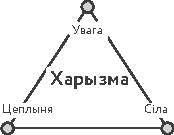
\includegraphics[scale=1.5]{willpower/ch9/10.pdf}
\end{figure}

\textbf{Увага}~--- найлепшы камплімэнт. Чым больш вы сфакусуецеся на суразмоўцы, тым больш харызматычныя будзеце, тым лепш зразумееце, гастрэй і эмацыйней зрэагуеце. Практыкуйце ўсьвядомленую камунікацыю: чалавек павінен ясна адчуваць, што ў~гэты момант ён для вас важнейшы за ўсё. Зьвяртайцеся да чалавека, выкарыстоўваючы словы ``вы'', ``вам'', ``ведаеце'' і да т.~п. Людзі счытваюць любое аслабленьне ўвагі да сваіх словаў і ацэньваюць вас нэгатыўна: чым мацней блукае ваш розум, тым больш адстаронена вы выглядаеце. Калі вы факусуецеся на сваіх эмоцыях і думках падчас гутаркі, то гэтае перажываньне выкідвае вас з~плыні. Давайце суразмоўцу такую ўвагу, быццам ад гэтай размовы залежыць ваша жыцьцё. Калі вы размаўляеце па тэлефоне, то заплюшчыце вочы, каб максімальна засяродзіцца на голасе. Падтрымлівайце кантакт і невэрбальна, асабліва важны для гэтага зрокавы кантакт. Разьвітваючыся, на тры сэкунды затрымайце позірк на суразмоўцы.

\textbf{Цеплыня}~--- гэта пазітыўнае ўспрыманьне іншага чалавека, павага яго асабістых межаў, поглядаў, пазьбяганьне крытыкі. Калі мы ўдзячныя чалавеку, добразычлівыя да яго, спачуваем яго праблемам і даём яму магчымасьць адчуць сябе значным, то гэта павялічвае нашу харызматычнасьць. Каб ваша цела і голас адбілі цеплыню, знайдзіце тры рэчы, якія вам падабаюцца ў~чалавеку, падумайце, чаму ён вас можа навучыць, падумайце аб перажытых ім пакутах.

\emph{Уявіце сабе ўсьмешлівае дзіця, калі гаворыце, тады ў~вашым голасе зьявіцца цеплыня.}

Сутнасьць цеплыні ў~тым, каб дазволіць людзям зрабіць на вас уражаньне, а~не наадварот. Важна зьвяртацца да ``лепшай версіі'' чалавека, чакаючы ад яго высокіх вынікаў і выяўляючы ўпэўненасьць, што ў~яго ўсё атрымаецца. Ня бойцеся паказаць і свае слабасьці, бо любы чалавек слабы, і гэта ў~вас агульнае. Цеплыня з~вашага боку дазваляе іншым выказаць сваю зацікаўленасьць у~вашых посьпехах, а~не зайздрасьць. Пакажыце, што гэтыя людзі, так ці інакш, зрабілі ўклад у~ваша прасоўваньне, пытайце меркаваньне іншых людзей, прасіце іх зрабіць невялікую ласку для вас.

\textbf{Сіла}~--- гэта валоданьне рэсурсамі і магчымасьцямі і гатоўнасьць іх ужываць. Упэўненасьць у~сабе, бачаньне будучыні і трансьляцыя яго навакольным, натхненьне, сьмеласьць і рашучасьць, упэўненасьць у~сабе паказваюць вашу сілу. Ваш статус, адзеньне, званьне~--- усё гэта ўплывае на ўспрыманьне сілы, але невэрбаліка, мабыць, галоўны яе кампанэнт. Цялесны, псыхалягічны дыскамфорт зьмяншаюць вашу прывабнасьць. Пазьбягайце хапатлівых рухаў, лішніх гэстаў, частых кіўкоў галавой, шматслоўя, нецярплівасьці, хваляваньня, словаў-паразітаў. Нэрвознасьць забівае харызму: спакой і стрыманасьць, паўзы ў~маўленьні, плястычныя рухі ўспрымаюцца як паказьнік сілы і статуту.

\subsection*{Пытаньні і заданьні}

1. Наколькі вы ўважлівыя да суразмоўцы? Выявіце максімум засяроджанасьці на ім.

2. У чым вы сёньняшні пераўзыходзіце сябе ўчорашняга?

3. Як вы можаце палепшыць свой гардэроб і свой стыль?


\section{Ікігай. Навошта вы гэта робіце?}

Старажытныя грэкі былі людзьмі, апантанымі войнамі, дэмакратыяй, адукацыяй, спортам, навукай і мастацтвам. Але на сьцяне іх галоўнага храма было напісана: «Спазнай самога сябе». Самапазнаньне яны лічылі нават важнейшым, чым здароўе. Жорсткае XX стагодзьдзе давяло справядлівасьць гэтай думкі.

\infobox{Самымі жыцьцеўстойлівымі ў~канцэнтрацыйных лягерах былі людзі з~высокім пачуцьцём уласнае годнасьці і разьвітой самаідэнтыфікацыяй: арыстакраты, кадравыя ваенныя, палітычныя і рэлігійныя зьняволеныя. Тыя, хто добра разумеў і ведаў, хто яны і дзеля чаго жывуць.}

Навукоўцы, якія вывучаюць доўгажыхароў, высьветлілі, што акрамя біялягічных прычын для здароўя і даўгалецьця вельмі важная асабістая ўсьвядомленасьць. У японцаў гэта завецца «ікігай» -- адчуваньне ўласнага прызначэньня ў~жыцьці. Цяпер ужо вядома, што фэномэн самасьвядомасьці зьвязаны з~адмысловымі верацёнападобнымі клеткамі ў~нашым мозгу, іх колькасьць карэлюе з~узроўнем усьвядомленасьці і здароўя. Гэтыя клеткі зьяўляюцца злучным зьвяном паміж кантролем за ўнутранымі функцыямі арганізма і вышэйшымі псыхічнымі працэсамі. Таксама яны ўдзельнічаюць у~фармаваньні кагнітыўных працэсаў, напрыклад пачуцьця «ўнутранага я», і зьяўляюцца цэнтральным участкам апрацоўкі нэрвовых сыгналаў, зьвязаных з~пастаноўкай мэтаў. Кажучы прасьцей, чым вышэй ваш узровень самаідэнтычнасьці і самаўсьвядомленасьці, тым вы больш жыцьцеўстойлівы і здаровы чалавек.

Як казаў Ніцшэ, «той, хто ведае ``навошта'', пераадолее любое ``як''». У нядаўнім мінулым мы дастаткова скептычна ўспрымалі «пошук сэнсу жыцьця». Сёньня ж можам упэўнена сьцьвярджаць, што сэнс~--- гэта навукова даказаны рэсурс здароўя, які можна і трэба прапампоўваць. Асэнсаванасьць жыцьця, мэты, пачуцьцё кірунку, ікігай~--- гэта ўсьвядомленае выманьне сэнсу са свайго паўсядзённага досьведу і сьвядомыя намеры, якія кіруюць нашымі паводзінамі.

\emph{Наяўнасьць мэты ў~жыцьці~--- магутны чыньнік яе падаўжэньня, акрамя таго, істотна запавольвае зьніжэньне кагнітыўных функцый (рызыка хваробы Альцгаймэра ў~2,5 разы ніжэй) незалежна ад іншых чыньнікаў.}

Акрамя аддаленых рызык, асэнсаванасьць пазітыўна ўплывае і на самаадчуваньне, напрыклад, чым больш асэнсаванае ваша жыцьцё, тым мацней і эфэктыўней вы сьпіце. І ня варта адразу пачынаць мучыцца пытаньнямі аб паходжаньні сусьвету, зрабіце свае разважаньні больш прадметнымі. Спытайце не ``нашто'', а~``на што'' вы прыйшлі ў~гэты сьвет, а~таксама ``для чаго'' і ``для каго''. Усьвядомлена паглядзіце на свае штодзённыя дзеяньні і задайце сабе тыя ж пытаньні. Не заўсёды адказы на іх будуць прыемнымі, але гэта тое, што напэўна варта пачаць рабіць. Адваротны бок сэнсу~--- гэта дасьледаваньне сябе, пошук сваёй самаідэнтычнасьці.

\begin{figure}[htb!]
  \centering
  
\includegraphics[scale=1.5]{willpower/ch9/11.pdf}
\end{figure}

\textbf{Самаідэнтычнасьць}~--- гэта ваш адказ на пытаньне ``хто я?''. Цяпер пытаньне самаідэнтычнасьці і самапазнаньня вельмі актуальнае, бо крызіс сучаснага сьвету шмат у~чым~--- гэта крызіс ідэнтычнасьці. Масавая вытворчасьць прывяла да стандартызацыі мноства рэчаў, ад прадуктаў да ідэй. Разбурэньне сямейных сувязяў, псэўдадухоўнасьць, імітацыя ўражаньняў і прадметаў, разбурэньне лякальных культур~--- асабліва актыўна дэіндывідуалізацыя шчыравала ў~таталітарных рэжымах, дзе адбывалася абязьлічваньне сем'яў, гарадоў і краін, а~цяпер гэтую ролю ўзялі на сябе вэстэрнізацыя і глябалізацыя ў~горшым сэнсе гэтага слова.

\infobox{Калі ў~стандартызацыі рэчаў ёсьць свае плюсы, напрыклад таннасьць, то стандартызацыя людзей таксама робіць іх ``таньнейшымі''.}

Спрабуючы кампэнсаваць \textbf{экзістэнцыйны вакуум}, людзі шукаюць сваю самаідэнтычнасьць. Рост нацыяналізму, рэлігійнасьці~--- гэта прыкметы браку самаідэнтычнасьці, бо людзям жыцьцёва важна сябе вызначыць, важна ``кімсьці быць''. Прамысловыя брэнды, дзяржавы, рэлігіі дзеюць аднолькава: яны ствараюць калектыўныя ідэнтычнасьці, да якіх чалавек ``належыць'' і якія ён нібыта павінен абараняць мацней, чым свае асабістыя інтарэсы. Але яны ніколі не сфарміруюць вашу сапраўдную асобу. Апранаючы на сябе гатовыя ролі, мы толькі фармуем фальшывую самаідэнтычнасьць, і гэта абмяжоўвае нашы магчымасьці, паралізуе нашы рэсурсы.

\textbf{Фальшывая ідэнтычнасьць} фармуецца, калі чалавек вызначае сябе адно сваёй біяграфіяй, увесь час адсылаючы сябе ў~мінулае і параўноўваючы зь ім. Або калі чалавек ідэнтыфікуе сябе з~групай, якой належыць, напрыклад: мужчына, француз, мэханік, футбольны фанат,~--- пераймаючы стандарты групы як уласныя. Часам фальшывай ідэнтычнасьцю можа быць імкненьне існаваць у~поўнай аўтаноміі і жыць толькі па сваіх законах па-за грамадствам. Маркетынг навязвае нам фальшывую ідэнтычнасьць ``індывідуальнасьці'', калі мы можам купіць мноства розных прадметаў і стварыць свой асабісты набор зь іх.

\textbf{Што рабіць?} У першую чаргу варта крытычна ставіцца да любой гатовай самаідэнтычнасьці. Гэта як зь ежай: усе ведаюць, чым небясьпечны фастфуд і што самая бясьпечная, карысная і смачная ежа~--- зробленая дома. Так і самаідэнтычнасьць~--- яе трэба вырошчваць і разьвіваць. Калі мы галодныя, мы часта ямо абы-што, а~калі мы ня верым і ня ведаем сябе, то гатовыя прыняць любую ідэнтычнасьць. Страта прыналежнасьці~--- гэта моцны стрэс, і мы гатовыя верыць у~што заўгодна, абы здабыць нейкую ўстойлівасьць. Таму людзі з~аслабленай самаідэнтычнасьцю, «бяспамятныя», так лёгка ўнушальныя і схільныя прапагандзе. Але як няма здаровага фастфуду, так няма і ўнівэрсальнай самаідэнтычнасьці. Яе немагчыма купіць у~краме, праца над яе стварэньнем запатрабуе ад вас значнага ўкладаньня часу і энэргіі, самае галоўнае ў~гэтым пошуку~--- працягваць шукаць.

\begin{figure}[htb!]
  \centering
  
\includegraphics[scale=1.5]{willpower/ch9/12.pdf}
\end{figure}

\emph{\textbf{Што вы пра сябе ведаеце?} Да якога калена вы ведаеце свой радавод? Між іншым, веданьне сваіх каранёў~--- гэта адзін з~важных аспэктаў самаідэнтычнасьці. Што вы ведаеце аб месцы, дзе жывяце? Вы ведаеце свае слабыя бакі? Як вы іх абараняеце? У чым вашыя моцныя бакі? Як вы іх карыстаеце? Што вы ўмееце рабіць? Што вы ўмееце рабіць лепш за калег? Што вам сапраўды падабаецца і чаму?}

\textbf{Калі вашыя веды пра сябе малыя, пачніце з~простага пытаньня: «Чым я заняты, калі мне падабаецца, хто я?» У канчатковым выніку, гэтыя і падобныя пытаньні дапамогуць вам адказаць на галоўнае пытаньне: «Хто я і чым адрозьніваюся ад іншых?»}

Тое, як вы адказваеце на гэтае пытаньне, шмат у~чым вызначае ваша здароўе. Немагчыма спазнаць сябе, застаючыся нерухомым. Старажытныя грэкі лічылі, што спазнаць сябе~--- значыць выпрабаваць сябе. Любое спазнаньне~--- гэта падарожжа. Вы можаце вывучаць любыя незнаёмыя рэчы, капаць ўшыркі, углыб, у~бакі. Спазнаючы новае пра сябе, мы дадаём частку сябе. І гэта тычыцца ня толькі розуму, але й цела. Чым вышэй у~вас узровень самаўсьвядомленасьці, чым лепш вы сябе ведаеце, тым лепшы выбар вы зможаце рабіць у~любых сытуацыях і атрымліваць ад яго нашмат больш задавальненьня. \textbf{Бо здароўе~--- гэта здаровае задавальненьне сваіх, сапраўдных, а~не чужых патрэбаў.}

\emph{Як добра заўважыў філёзаф Раман Кразнарык, «мы ўвайшлі ў~эпоху новага багацьця, пры якім сэнс таго, што ты робіш, становіцца даражэйшым за грошы».}

Цяпер недастаткова зрабіць проста харошы прадукт, патрэбны ўнікальны прадукт, а, застаючыся ўсераднёным, гэтага дасягнуць немагчыма. Дрэву для шырокай кроны патрэбныя глыбокія карані, так і чалавеку для вонкавых праяў патрэбныя разьвітыя самаўсьвядомленасьць і самаідэнтычнасьць. Будзьце адданыя ня вонкавай ідэі, а~самому сабе~--- і гэта зробіць вас здаравейшымі й больш пасьпяховымі. Калі ад чужой ідэі лёгка адкаснуцца, то сапраўднае, ваша асабістае пакліканьне будзе заўсёды вас натхняць.

Некаторыя навукоўцы лічаць, што гонар за сваё паходжаньне зьяўляецца важным кампанэнтам посьпеху. Калі чалавек упэўнены зь дзяцінства, што ён пераўзыходзіць іншых, то гэтая вера будзе дапамагаць яму праяўляць свае якасьці. Існае пачуцьцё ўласнае перавагі неабходна падмацоўваць і даводзіць на практыцы, таму, калі дадаць да яго некаторую ўпэўненасьць у~сабе,~--- гэта дапаможа дамагацца посьпеху. А ў~спалучэньні са здольнасьцю да кантролю імпульсаў, г.~зн. дысцыплінай, гэтая імавернасьць становіцца яшчэ вышэй.

\subsection*{Асабісты брэнд, або Стварыце сабе імя}

Вашы рашэньні адносна стылю, захапленьняў, адзеньня і да т.~п., у~ідэале павінны адлюстроўваць вашыя каштоўнасьці і служыць павышэньню вашай пазнавальнасьці. Імя-брэнд адразу зьяўляецца гарантам якасьці, выклікае давер, прыцягвае, інфармуе.

\emph{Як дакладна сказаў заснавальнік Amazon Джэф Бэзас: ``Асабісты брэнд~--- тое, што пра вас кажуць людзі, калі вас няма ў~пакоі''.}

У аснове асабістага брэнда ляжаць тры ключавыя паняцьці: прафэсіяналізм, рэпутацыя і папулярнасьць. Калі чагосьці з~гэтага бракуе, то сфармаваць асабісты брэнд будзе складана. Чым бы вы ні займаліся, будзьце сумленнымі. Разьвівайцеся як прафэсіянал, заявіце пра сябе і будзьце навідавоку, пішыце артыкулы, выступайце на тэлебачаньні, давайце гострыя і актуальныя камэнтары на важныя тэмы. Пры гэтым лепш рэклямуйце сваю справу, а~не імя. Нават калі вы працуеце ў~кампаніі, памятайце, што спачатку людзі давяраюць чалавеку і толькі потым~--- фірме, так за Amazon стаіць Джэф Бэзас, за Apple~--- Стыў Джобс, за Microsoft~--- Біл Гейтс. Як вашыя звычкі, адзеньне, сацсеткі, сайт, інтэрвію адлюстроўваюць ваш асабісты брэнд? Ці ёсьць у~гэтым цэльнасьць?

\begin{figure}[htb!]
  \centering
  
\includegraphics[scale=1.5]{willpower/ch9/13.pdf}
\end{figure}

Як мы ўжо даведаліся, сацыяльны статус шмат у~чым вынікае з~унутраных адчуваньняў, і няма сэнсу шукаць яго звонку. Мы каштоўныя тым, што ствараем карысныя для іншых людзей каштоўнасьці, што мы важныя для іншых людзей. Гатовыя адказы на пытаньні аб сэнсе жыцьця, якія прапануюць розныя вучэньні, маюць шмат пабочных эфэктаў.

\textbf{Пошук гэтых адказаў~--- толькі наша асабістая справа, стварэньне каштоўнасьцяў~--- толькі наша асабістая справа.} Тое, як мы выкарыстоўваем сваё жыцьцё і ў~што ператвараем свой гадзіньнік,~--- і ёсьць сэнс. Ён заключаны ў~рэальнасьці і ў~тым, як мы можам выкарыстоўваць яе ў~сваіх мэтах. Адаптуючыся, дзейнічаючы ўважліва і гнутка, мы дасягаем сваіх мэтаў. Чакаць, што рэальнасьць зьменіцца, каб адпавядаць нашым уяўленьням пра яе, -- глупства, але гэтым занятыя безьліч людзей. 

\emph{Думайце над тым, як дзейнічаць і якія задачы вырашаць, а~не спэкулюйце думкамі для тлумачэньня сваіх няўдач або пошуку апраўданьняў.}

\subsection*{Як знайсьці ікігай?}

Чым лепей мы сябе ведаем, прымаем свае рысы і асаблівасьці, тым лепшыя рашэньні прымаем. Важна вызначыць свае моцныя і слабыя рысы, свае крыніцы энэргіі і матывацыі, радасьці і задавальненьняў, зразумець, што прыводзіць нас у~стан плыні, якія ў~нас ёсьць чаканьні ад сябе і ад іншых. Падумаць, што трэба ў~грамадстве, што найбольш запатрабавана? 

\infobox{Ікігай~--- гэта ня проста вашае жаданьне, а~тое, што знаходзіцца на скрыжаваньні чатырох сфэраў: за што добра плацяць, што вы ўмееце рабіць, што вам падабаецца і што трэба людзям.}

Некаторыя аўтары вылучаюць наступныя найважнейшыя чыньнікі ўсьвядомленай кар'еры: прыбытак, статус, выкарыстаньне талентаў, разуменьне значнасьці сваёй працы, задавальненьне.

\textbf{Працягвайце пытацца ў~сябе і назіраць.} Што для вас самае каштоўнае? Чым ганарыцеся? Што ўмееце рабіць? У чым вы прафэсіянал? Якія навыкі трэба паляпшаць? Што вы любіце рабіць? Ад чаго замірае сэрца? Аб чым марыце? Што павышае вашу самаацэнку? Хто вы ў~марах? Чаго вы чакаеце ад працы~--- калектыў, дасягненьні, кар'ера, грошы? Спытайце сябе шчыра: я падабаюся сабе, калі раблю гэта? Ці падабаецеся вы сабе раздражнёным, лежачы на канапе і купляючы тавары па акцыі? А зараз падумайце, чым вы бываеце занятыя, калі вам падабаецца, хто вы такі. Калі вы расьцяце, калі вы перамагаеце?

\textbf{Гэта нармальна~--- шукаць сваё шчасьце і пакліканьне.} Вы нікому нічога не павінны рабіць, калі гэта не прыносіць вам шчасьця і задавальненьня ад жыцьця. Назапасьцеся цярпеньнем, бо ваш пошук можа заняць доўгі час, і самае важнае ў~ім~--- працягваць шукаць і дзейнічаць. Схадзіце ў~кнігарню, пагартайце кнігі ў~розных разьдзелах. Спытайце сябе, у~якім разьдзеле вы б хацелі прачытаць усё? Успомніце людзей, якім вы зайздросьцілі і якіх пераймалі. Чым яны займаліся? Што вы любілі ва ўзросьце 13--15 гадоў? У якой справе вы з~задавальненьнем бралі звышмерную працу ці гатовыя былі займацца гэтым бясплатна?

\subsection*{Самаацэнка і годнасьць}

Часта людзі спрабуюць павышаць сваю самаацэнку штучна, а~не праз павелічэньне сваіх рэсурсаў. Напампоўваньне ілюзій прыводзіць толькі да завышэньня прэтэнзій да навакольнага сьвету і павялічвае рызыку дэпрэсіі. Сьцьвярджаць сабе, што вы самы разумны,~--- ня зробіць вас разумнейшым. Зьмена самаўяўленьня адбываецца ў~выніку дзеяў, а~не разважаньняў. Наш мозг, назіраючы за тым, што мы робім, мяняе нашу самаацэнку і ўяўленьні пра сябе. Калі вы баіцеся, але дзейнічаеце адважна, робіце гэта ўвесь час, то вы пачынаеце думаць пра сябе як пра адважнага чалавека.

\textbf{Дзеяньне мяняе ўяўленьне, а~не наадварот.} Прычына высокай самаацэнкі~--- перамогі і спрыяльныя падзеі ў~жыцьці чалавека. Для здаровай самаацэнкі важна параўноўваць сябе цяперашняга з~сабой у~мінулым, а~пры параўнаньні зь іншымі людзьмі параўноўваць сябе з~адэкватнай рэфэрэнтнай групай: чаго дамагліся людзі майго ўзросту за гэты тэрмін. Важна ў~любой сытуацыі захоўваць годнасьць~--- гэта наша каштоўнасьць, павага да сябе, аўтаномія, удзел у~прыняцьці рашэньняў і свабода выбару. Захоўваць гонар і самапавагу~--- важныя рысы статусу і пазітыўнае адчуваньне ўласнае каштоўнасьці.

\textbf{Будзьце найлепшымі ў~тым, што вы робіце.} У японцаў ёсьць яшчэ адно паняцьце~--- кодавары, яно абазначае адказны падыход да сваёй справы. Гэта ваш асабісты прафэсійны стандарт, калі вы ўвесь час удасканальваецеся, выяўляючы ўвагу нават да самых дробных дэталяў і дамагаючыся ідэальных вынікаў.

\textbf{Выбірайце тую справу, якая атрымліваецца, і ўдасканальвайцеся, становячыся лепшымі. Адчуваньне росту і перавагі~--- гэта тое, што павышае ваш статус і самаацэнку.}

Факусуючыся на сваіх моцных баках, вы атрымліваеце імпульс да росту. Калі ў~здароўі карысна закрываць свае слабыя бакі ў~першую чаргу, то ў~выпадку са статутам усё наадварот~--- адна ваша яркая рыса або талент важнейшыя за сотню слабасьцяў. Разьвівайце свае наймацнейшыя бакі, і яны кампэнсуюць усё астатняе. Адчуваньне прагрэсу і значнасьці матывуе~--- калі мы становімся лепш і лепш у~тым, што для нас вельмі важна, калі мы служым глябальным мэтам, якія пераўзыходзяць нашы патрэбы.

Статус шчыльна зьвязаны са стварэньнем і захаваньнем вашага ўнутранага кодэксу. Не вашыя эмоцыі кіруюць вашым жыцьцём, а~вашыя каштоўнасьці і прынцыпы вызначаюць тое, як вы разьмяркоўваеце свой час. Не стамляйцеся ў~сябе пытацца, ці правільныя рэчы вы робіце? Веданьне сваіх здольнасьцяў і талентаў, выкарыстаньне іх вельмі важнае ў~канкурэнтнай барацьбе.

\emph{Падумайце, у~якіх сфэрах жыцьця вы хочаце рабіць гэтыя рэчы, ці робіце вы іх натуральна, адчуваеце ў~працэсе задавальненьне і здавальненьне, лёгка вучыцеся, дзейнічаеце неардынарна і эфэктыўна нават пад ціскам?}

\subsection*{Пытаньні і заданьні}

1. У чым сэнс вашага жыцьця, на ваш погляд?

2. Ці ёсьць у~вас асабісты брэнд?

3. Ці добрыя вы ў~тым, што робіце? Ці хочаце стаць лепей?

\clearpage
\thispagestyle{empty}
\begin{figure}[htb!]
  \vspace*{-0.15in}
  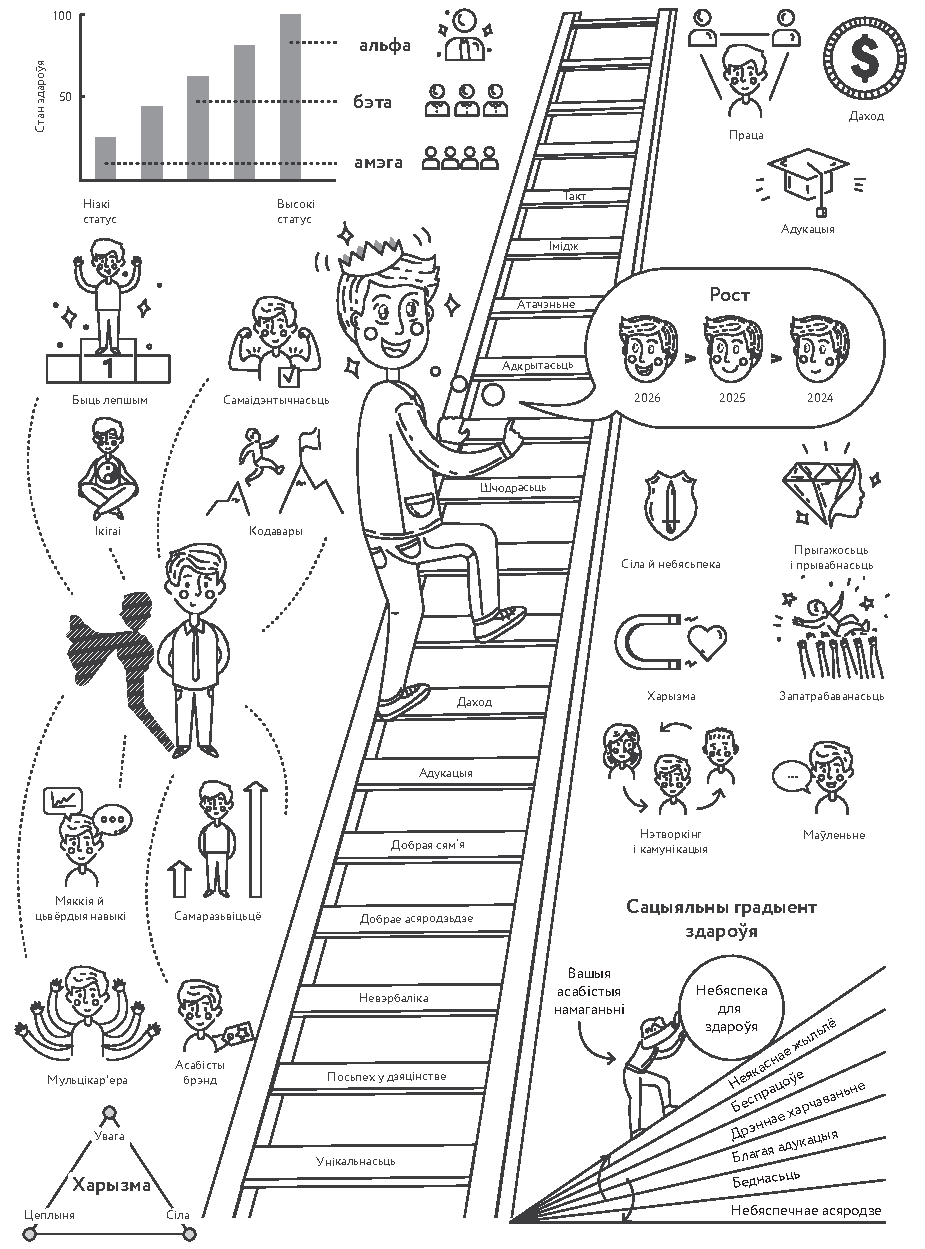
\includegraphics[width=\textwidth]{willpower/ch9/full.pdf}  
\end{figure}
